\documentclass[12pt]{article}
\usepackage[a4paper, hmargin=1in, bottom=1in, top=1in]{geometry}
\usepackage{graphicx}
\usepackage{booktabs}
\usepackage{caption}
\usepackage{float}
\usepackage{amsmath}
\usepackage{listings}
\usepackage{xcolor}
\usepackage{caption}
\usepackage{subcaption}

\lstset{
    basicstyle=\ttfamily\small,
    breaklines=true,
    keywordstyle=\color{blue},
    commentstyle=\color{gray},
    numbers=left,
    numberstyle=\tiny,
    frame=single,
    showstringspaces=false
}

\begin{document}

\begin{titlepage}
	\centering

	\huge \textbf{EE 671: VLSI Design} \\
	\vspace{1cm}

	\LARGE \textsc{Project 1} \\
	\vspace{4.5cm}

	
\includegraphics[width=0.55\textwidth]{../../icon.png} \\

	\vspace{4.5cm}

	\Large
	\begin{tabular}{rl}
		\textbf{Submitted by:}    & Bhuvansh Goyal (22B3908)   \\
		                          & Saarthak Krishan (22B3959) \\
		                          & Hardik Jangir (22B3901)    \\
		                          & Sambhavi Jaiswal (24D0545) \\
		\textbf{Instructor:}      & Prof. Laxmeesha Somappa    \\
		\textbf{Submission Date:} & 13 Sep 2025
	\end{tabular}

	\vfill
\end{titlepage}

\clearpage

\tableofcontents

\clearpage
\section{Cell: invx1}
\subsection{Circuit Diagram}
Figure~\ref{fig:invx1_circuit} shows the schematic of the invx1 cell.
\begin{figure}[H]
	\centering
	\includegraphics[width=0.4\textwidth]{./inv.eps}
	\caption{Circuit diagram of the invx1 cell}
	\label{fig:invx1_circuit}
\end{figure}

\subsection{Transistor Dimensions}
The width and length of the MOSFETs used in the cell are listed in Table~\ref{tab:inv_mosfet_dims}.

\begin{table}[H]
	\centering
	\begin{tabular}{|c|c|c|}
		\hline
		     & \textbf{Width ($\mu$m)} & \textbf{Length ($\mu$m)} \\
		\hline
		PMOS & 1.26                    & 0.15                     \\
		NMOS & 0.42                    & 0.15                     \\
		\hline
	\end{tabular}
	\caption{MOSFET width and length values for the invx1 cell}
	\label{tab:inv_mosfet_dims}
\end{table}

\subsection{Layout}
The layout of the invx1 cell is shown in Figure~\ref{fig:invx1_layout}. The cell area is measured as:
\[
	\text{Area} = 2.61 \mu \times 2.72 \mu = 7.099 \mu m^2
\]

\begin{figure}[H]
	\centering
	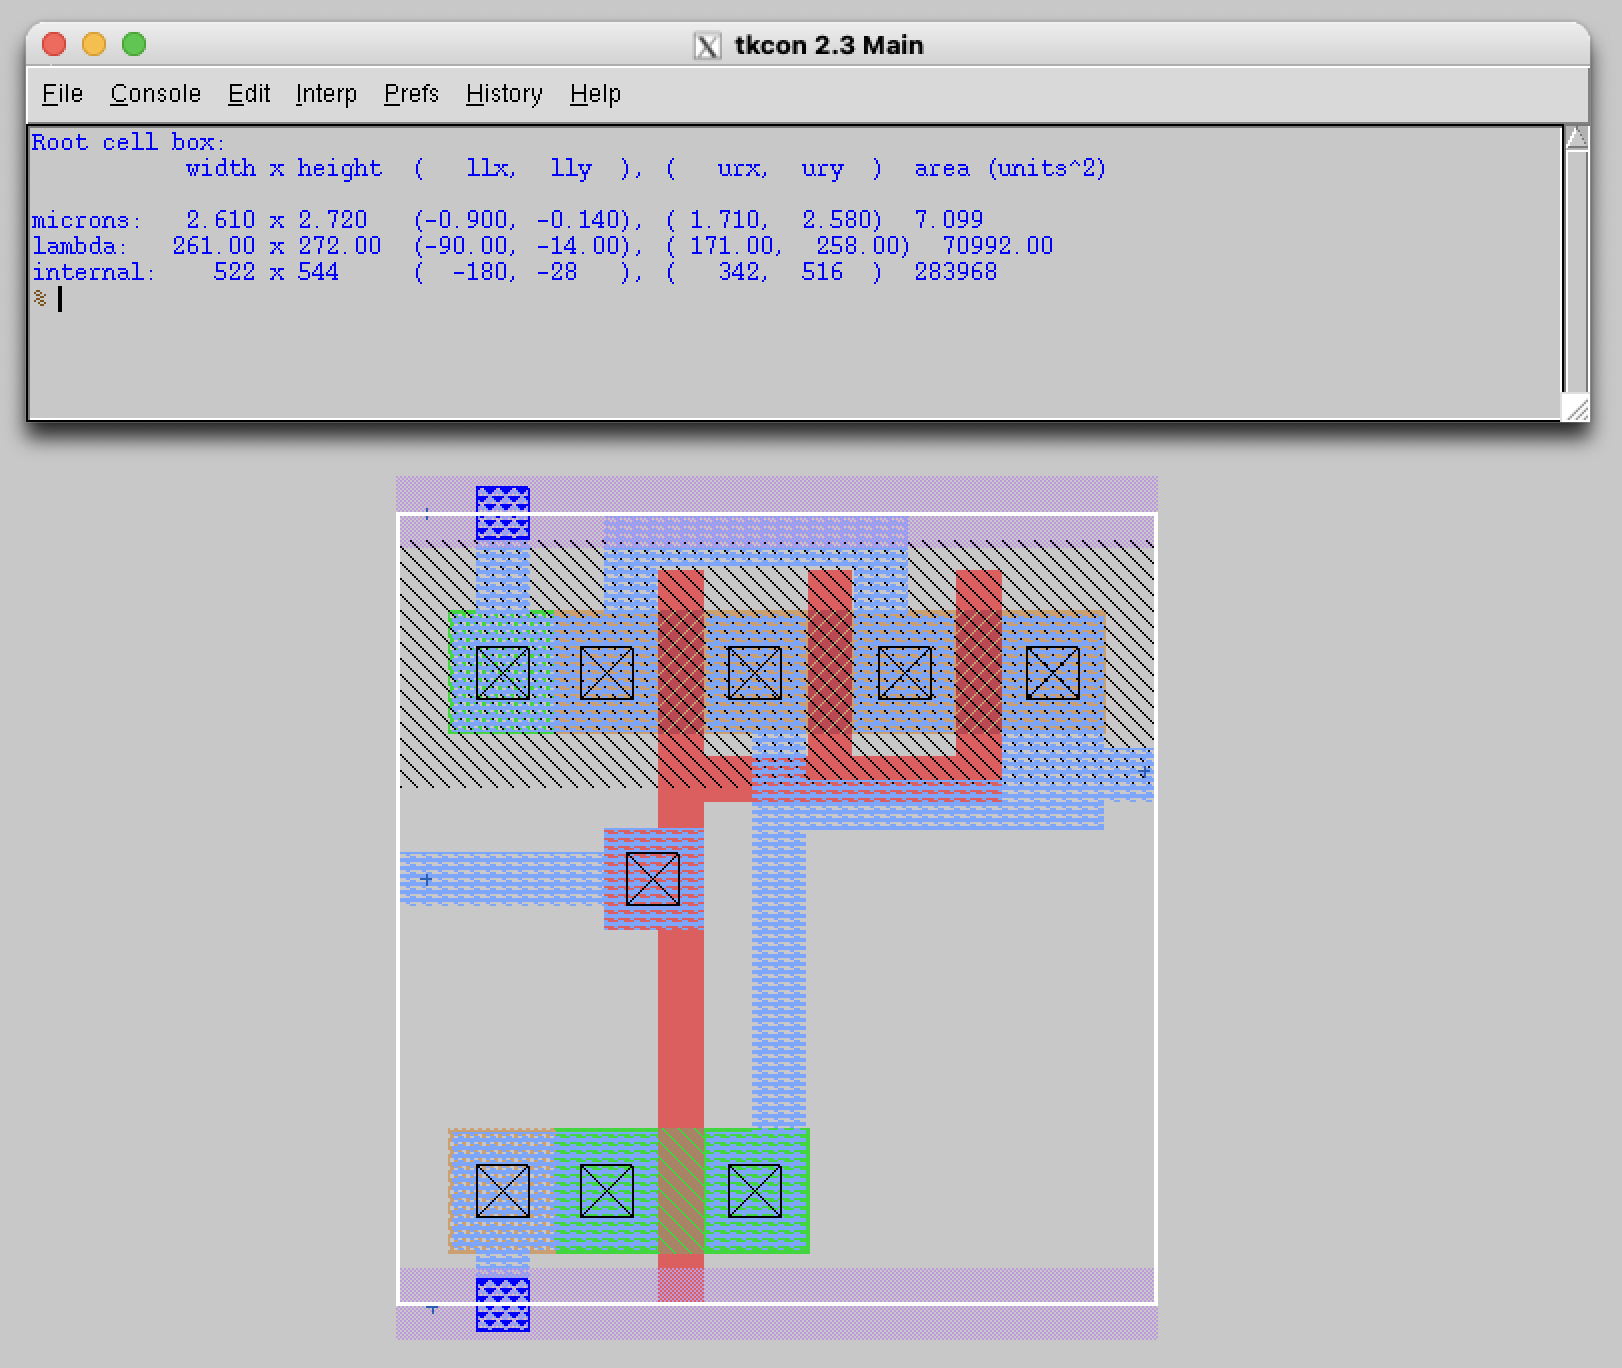
\includegraphics[width=0.7\textwidth]{./invx1_layout.png}
	\caption{Layout of the invx1 cell}
	\label{fig:invx1_layout}
\end{figure}

\subsection{Original Netlist}
The netlist written for the invx1 cell is shown below:
\lstinputlisting[language={}]{../dfxtn/ngspice_simulations/invx1_schematic.spice}

\subsection{PEX Netlist}
The extracted netlist of the cell is shown below:
\lstinputlisting[language={}]{../dfxtn/layout/invx1_layout_pex.spice}

\subsection{Verification}
The DRC and LVS results are clean (Figure~\ref{fig:invx1_verification}).

\begin{figure}[H]
	\centering
	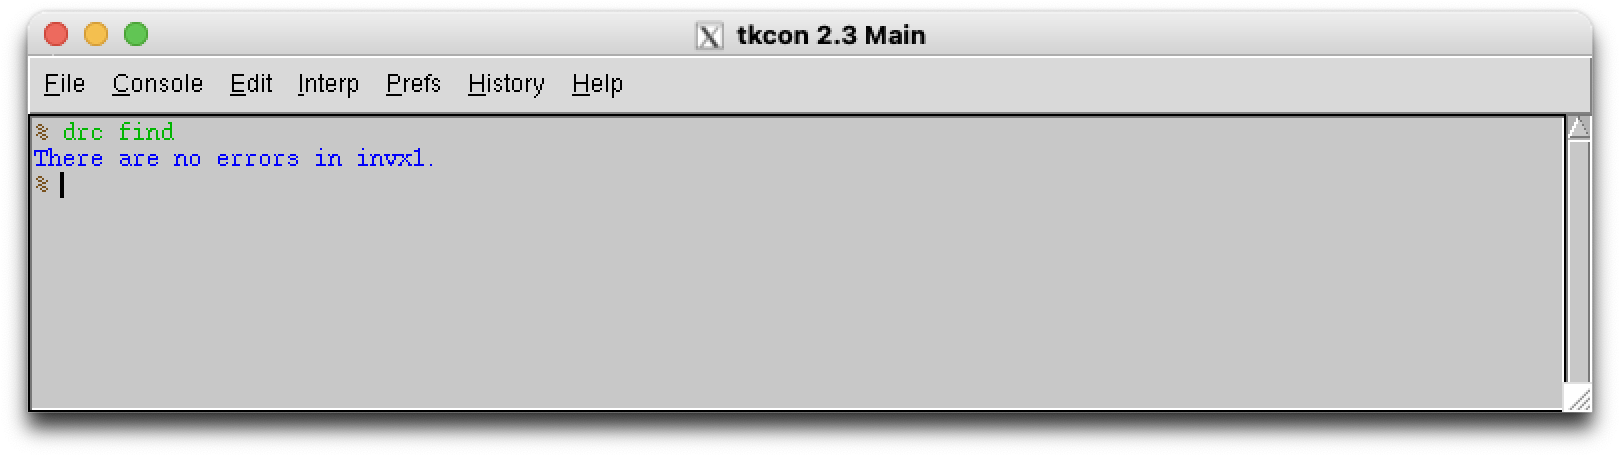
\includegraphics[width=0.45\textwidth]{./invx1_drc.png}
	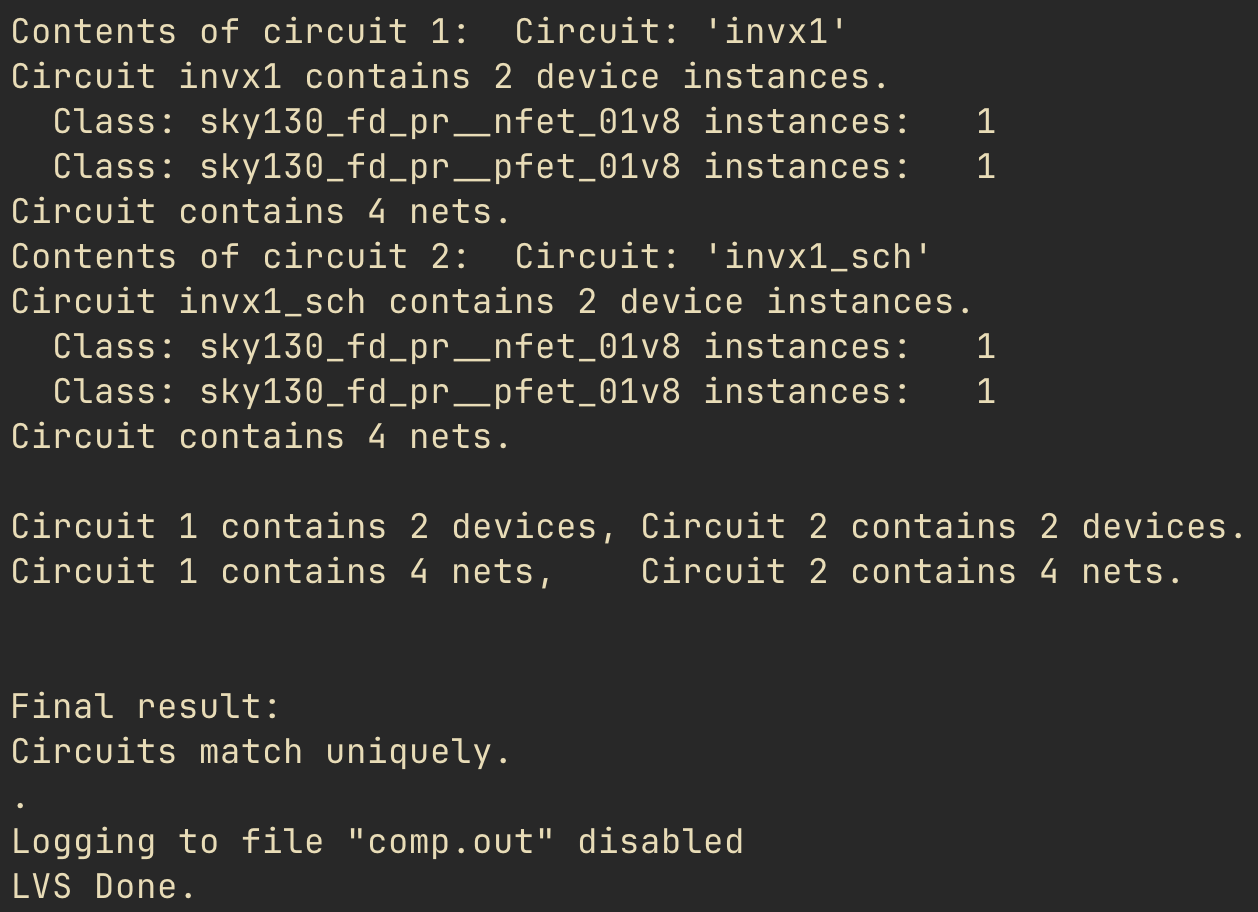
\includegraphics[width=0.45\textwidth]{./invx1_lvs.png}
	\caption{DRC and LVS clean results for the invx1 cell}
	\label{fig:invx1_verification}
\end{figure}

\subsection{Timing and Power Characterisation}
\subsubsection{Input Pin Capacitances}

\begin{table}[H]
	\centering
	\begin{tabular}{|c|c|c|c|}
		\hline
		\textbf{Input Pin} & \textbf{Rise Cap (fF)} & \textbf{Fall Cap (fF)} & \textbf{Average Cap (fF)} \\
		\hline
		A                  & 2.915                  & 2.915                  & 2.915                     \\
		\hline
	\end{tabular}
	\caption{Input pin capacitance values}
\end{table}

\subsubsection{Transition Time Tables}

\begin{table}[H]
	\centering
	\begin{tabular}{|c|c|c|c|}
		\hline
		                & \textbf{10 ps} & \textbf{100 ps} & \textbf{1000 ps} \\
		\hline
		\textbf{0.5 fF} & 0.014          & 0.023           & 0.084            \\
		\hline
		\textbf{10 fF}  & 0.066          & 0.068           & 0.173            \\
		\hline
		\textbf{100 fF} & 0.577          & 0.577           & 0.588            \\
		\hline
	\end{tabular}
	\caption{Output Rise Transition Time (ns) — Input Slew vs Output Capacitance (Related pin A, others held constant)}
\end{table}

\begin{table}[H]
	\centering
	\begin{tabular}{|c|c|c|c|}
		\hline
		                & \textbf{10 ps} & \textbf{100 ps} & \textbf{1000 ps} \\
		\hline
		\textbf{0.5 fF} & 0.014          & 0.021           & 0.084            \\
		\hline
		\textbf{10 fF}  & 0.073          & 0.073           & 0.174            \\
		\hline
		\textbf{100 fF} & 0.642          & 0.642           & 0.648            \\
		\hline
	\end{tabular}
	\caption{Output Fall Transition Time (ns) — Input Slew vs Output Capacitance (Related pin A, others held constant)}
\end{table}

\subsubsection{Propagation Delay Time Tables}

\begin{table}[H]
	\centering
	\begin{tabular}{|c|c|c|c|}
		\hline
		                & \textbf{10 ps} & \textbf{100 ps} & \textbf{1000 ps} \\
		\hline
		\textbf{0.5 fF} & 0.014          & 0.033           & 0.085            \\
		\hline
		\textbf{10 fF}  & 0.051          & 0.075           & 0.222            \\
		\hline
		\textbf{100 fF} & 0.399          & 0.423           & 0.658            \\
		\hline
	\end{tabular}
	\caption{Cell Rise Delay (ns) — Input Slew vs Output Capacitance (Related pin A, others held constant)}
\end{table}

\begin{table}[H]
	\centering
	\begin{tabular}{|c|c|c|c|}
		\hline
		                & \textbf{10 ps} & \textbf{100 ps} & \textbf{1000 ps} \\
		\hline
		\textbf{0.5 fF} & 0.018          & 0.034           & 0.078            \\
		\hline
		\textbf{10 fF}  & 0.065          & 0.085           & 0.216            \\
		\hline
		\textbf{100 fF} & 0.501          & 0.521           & 0.727            \\
		\hline
	\end{tabular}
	\caption{Cell Fall Delay (ns) — Input Slew vs Output Capacitance (Related pin A, others held constant)}
\end{table}

\subsubsection{Static Power}

\begin{table}[H]
	\centering
	\begin{tabular}{|c|c|}
		\hline
		\textbf{Condition (A)} & \textbf{Power (nW)} \\
		\hline
		0                      & 0.44                \\
		\hline
		1                      & 0.108               \\
		\hline
	\end{tabular}
	\caption{Static power dissipation under different input conditions}
\end{table}

\subsubsection{Dynamic Power Tables}

\begin{table}[H]
	\centering
	\begin{tabular}{|c|c|c|c|}
		\hline
		                & \textbf{10 ps} & \textbf{100 ps} & \textbf{1000 ps} \\
		\hline
		\textbf{0.5 fF} & 3857           & 3879            & 6690             \\
		\hline
		\textbf{10 fF}  & 19454          & 19304           & 20977            \\
		\hline
		\textbf{100 fF} & 150969         & 148418          & 158437           \\
		\hline
	\end{tabular}
	\caption{Dynamic Rise Power (nW) — Input Slew vs Output Capacitance (Related pin A, others held constant)}
\end{table}

\subsection{Verilog}

\subsubsection{invx1 Verilog Code}
The Verilog code for the invx1 cell used in simulations is shown below:

\lstinputlisting[language=Verilog, caption={invx1 Verilog code}, label={lst:invx1_verilog}]{../dfxtn/invx1.v}

\subsubsection{Testbench}
The Verilog testbench used to verify the invx1 functionality is shown below:

\lstinputlisting[language=Verilog, caption={invx1 Testbench code}, label={lst:invx1_tb}]{../dfxtn/tb_invx1.v}

\subsubsection{Simulation Waveform}
The waveform from the Verilog simulation showing the input, output, and clock signals is shown in Figure~\ref{fig:invx1_verilog_waveform}.

\begin{figure}[H]
	\centering
	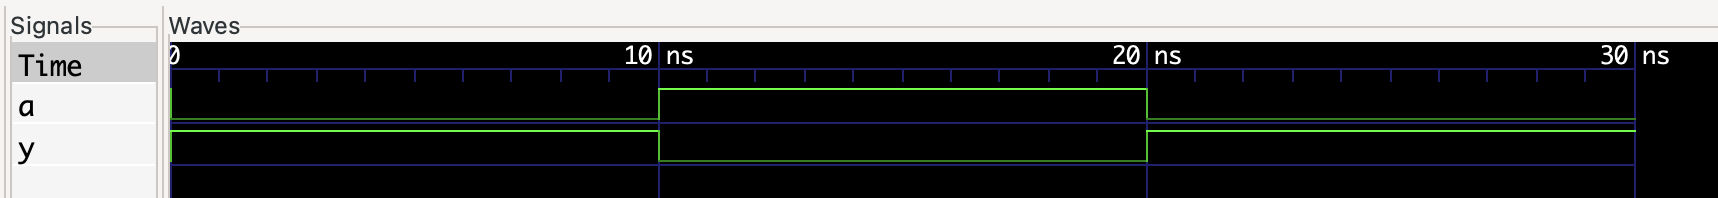
\includegraphics[width=0.8\textwidth]{./verilog_invx1.png}
	\caption{Verilog simulation waveform of the invx1 cell}
	\label{fig:invx1_verilog_waveform}
\end{figure}


\clearpage

\section{Cell: a21oi}
\subsection{Circuit Diagram}
Figure~\ref{fig:a21oi_circuit} shows the schematic of the a21oi cell.
\begin{figure}[H]
	\centering
	\includegraphics[width=0.4\textwidth]{./comb.eps}
	\caption{Circuit diagram of the a21oi cell}
	\label{fig:a21oi_circuit}
\end{figure}

\subsection{Transistor Dimensions}
The width and length of the MOSFETs used in the cell are listed in Table~\ref{tab:a21oi_mosfet_dims}.

\begin{table}[H]
	\centering
	\begin{tabular}{|c|c|c|}
		\hline
		                   & \textbf{Width ($\mu$m)} & \textbf{Length ($\mu$m)} \\
		\hline
		$\text{PMOS}_{A1}$ & 3                       & 0.15                     \\
		$\text{NMOS}_{A1}$ & 0.9                     & 0.15                     \\
		$\text{PMOS}_{A2}$ & 3                       & 0.15                     \\
		$\text{NMOS}_{A2}$ & 0.9                     & 0.15                     \\
		$\text{PMOS}_{B1}$ & 3                       & 0.15                     \\
		$\text{NMOS}_{B1}$ & 0.45                    & 0.15                     \\
		\hline
	\end{tabular}
	\caption{MOSFET width and length values for the a21oi cell}
	\label{tab:a21oi_mosfet_dims}
\end{table}

\subsection{Layout}
The layout of the a21oi cell is shown in Figure~\ref{fig:a21oi_layout}. The cell area is measured as:
\[
	\text{Area} = 9.93 \mu \times 2.72 \mu = 27.01 \mu m^2
\]

\begin{figure}[H]
	\centering
	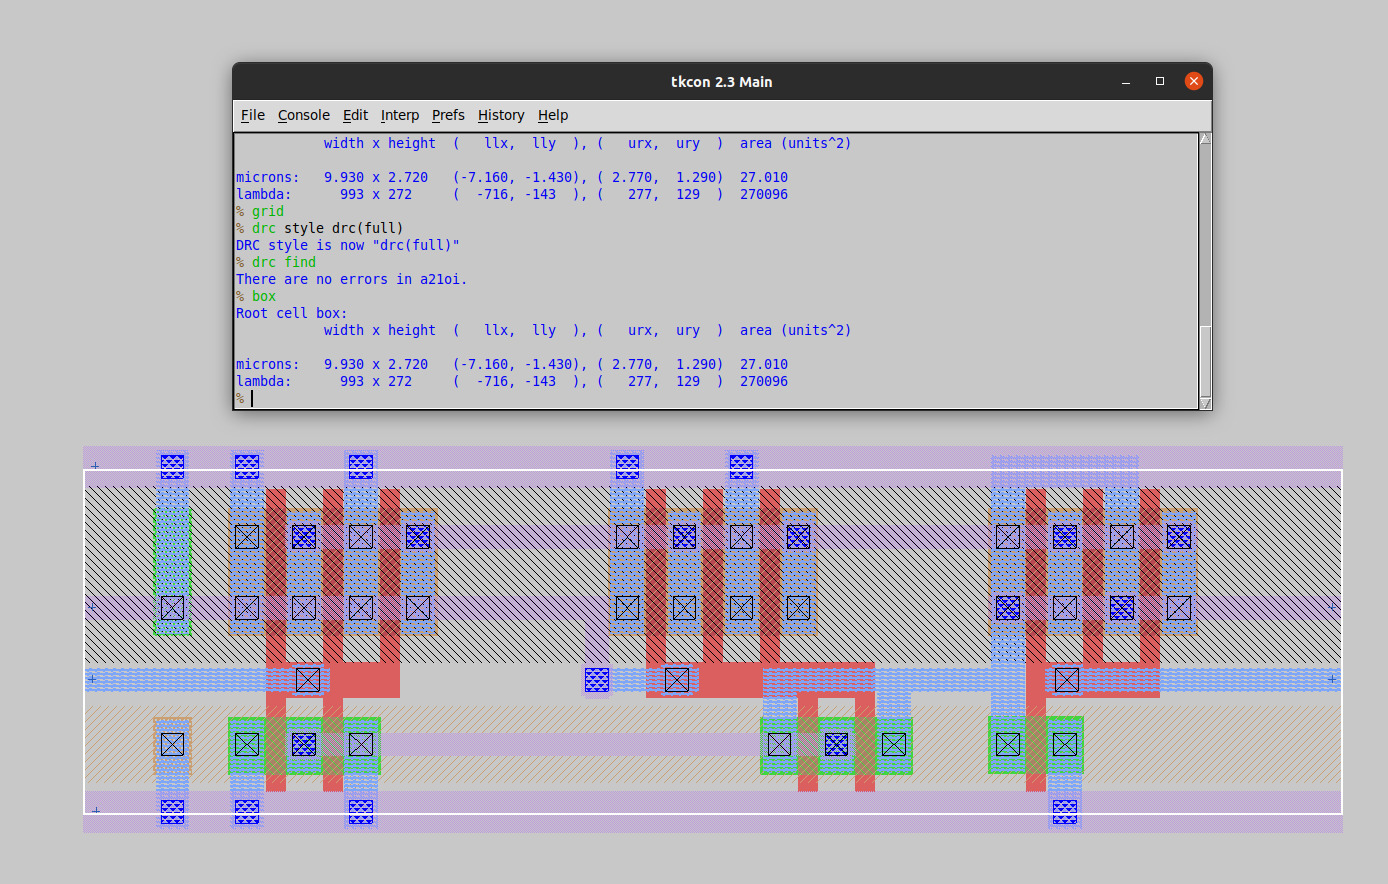
\includegraphics[width=0.7\textwidth]{./layout_a21oi.jpeg}
	\caption{Layout of the a21oi cell}
	\label{fig:a21oi_layout}
\end{figure}

\subsection{Original Netlist}
The netlist written for the a21oi cell is shown below:
\lstinputlisting[language={}]{../a21oi/ngspice_simulations/a21oi_schematic.spice}

\subsection{PEX Netlist}
The extracted netlist of the cell is shown below:
\lstinputlisting[language={}]{../a21oi/ngspice_simulations/a21oi_layout_pex.spice}

\subsection{Verification}
The DRC and LVS results are clean (Figure~\ref{fig:a21oi_verification}).

\begin{figure}[H]
	\centering
	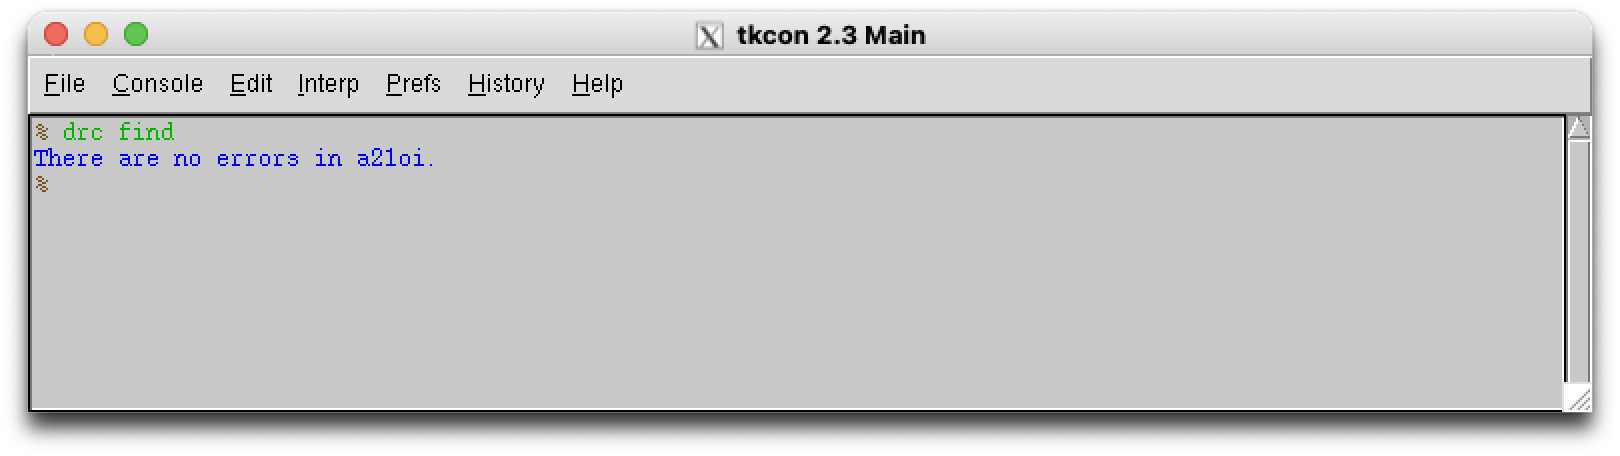
\includegraphics[width=0.45\textwidth]{./drc_a21oi.png}
	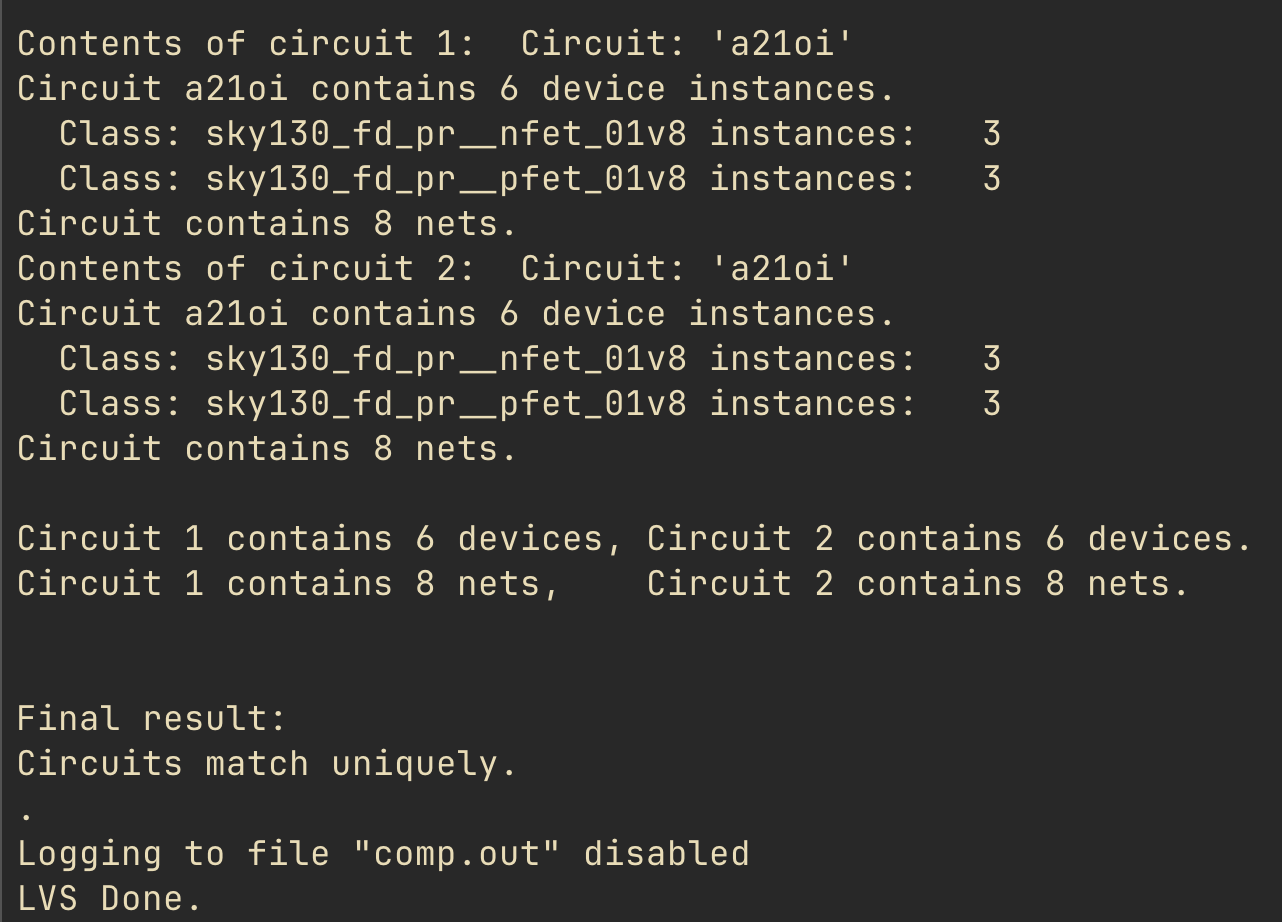
\includegraphics[width=0.45\textwidth]{./lvs_a21oi.png}
	\caption{DRC and LVS clean results for the a21oi cell}
	\label{fig:a21oi_verification}
\end{figure}

\subsection{Waveforms}

Shown below is one representative waveform ($a_2=1$, $b_1=0$, $a_1$ pulsing)
used to calculate $t_{rise}$, $t_{fall}$, and $t_{propagation}$.

\begin{figure}[H]
	\centering
	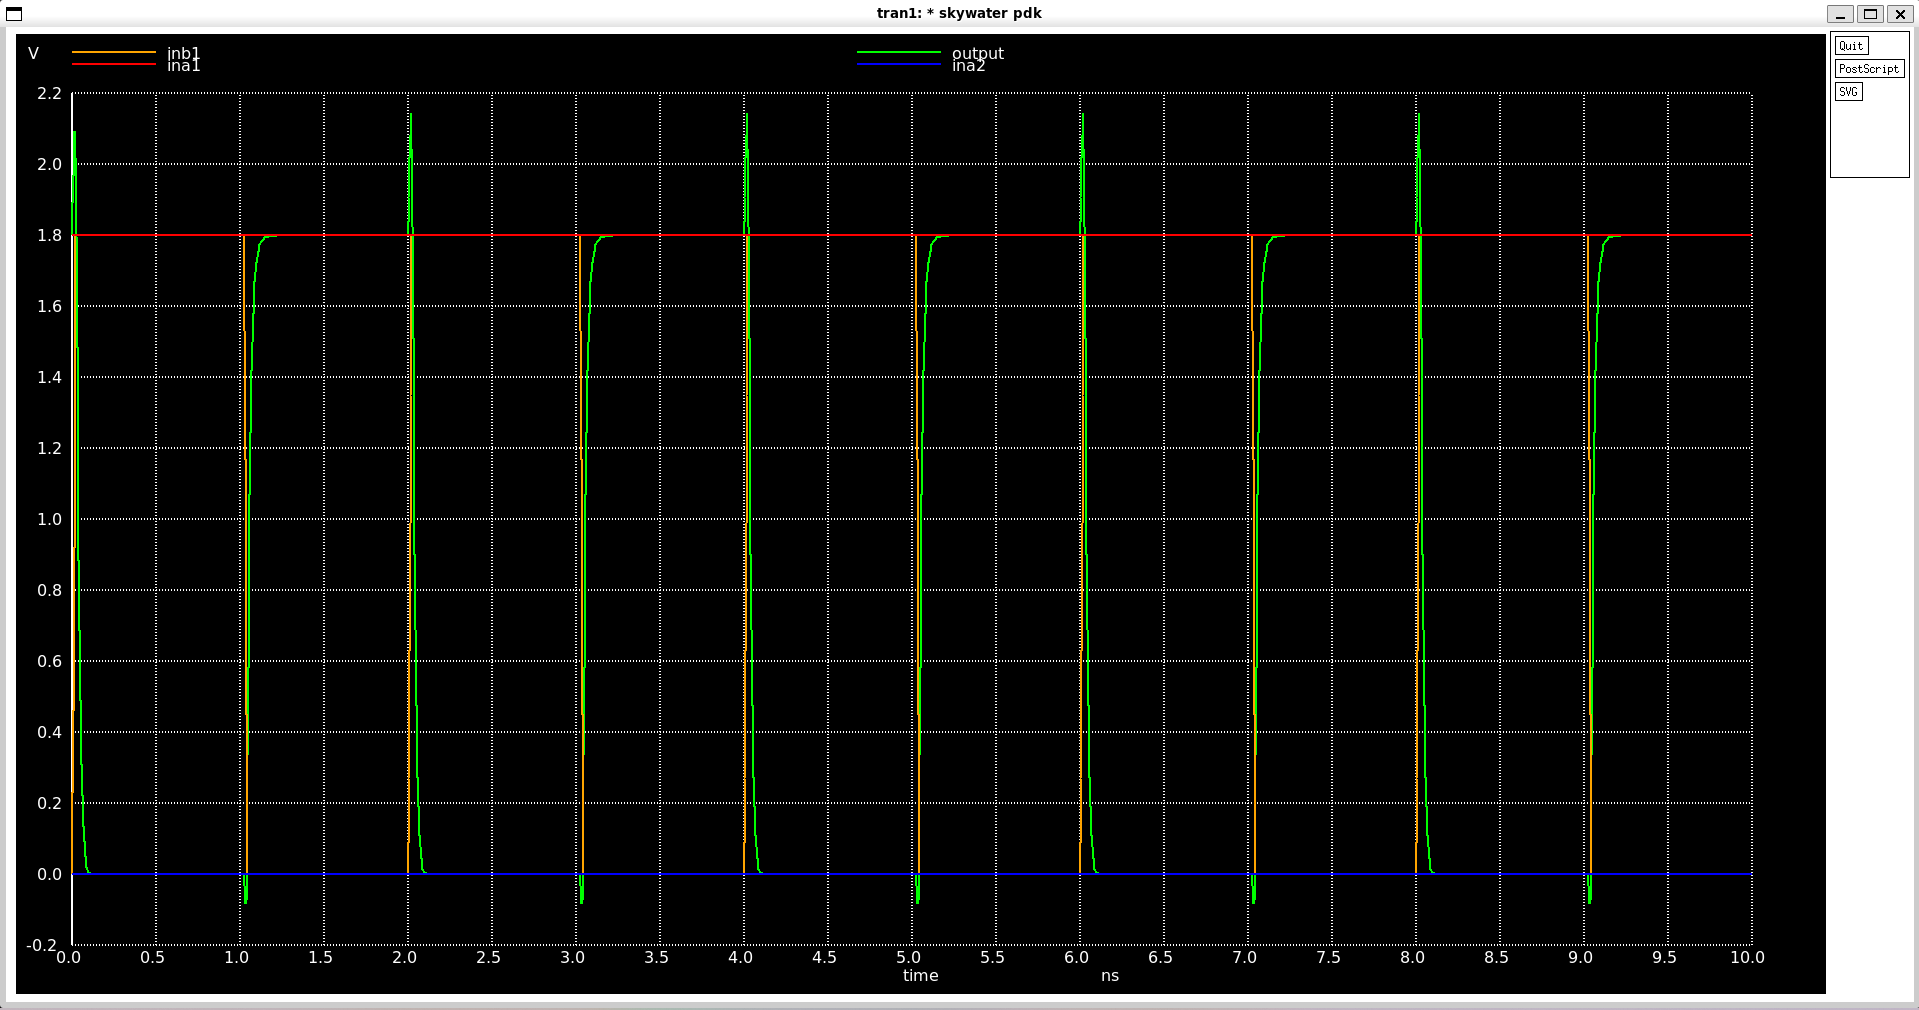
\includegraphics[width=0.85\textwidth]{./a21oi_waveform.png}
	\caption{Simulation waveform for $a_2=1$, $b_1=0$, $a_1$ pulsing}
\end{figure}

\subsection{Timing and Power Characterisation}

%%%%%%%%%%%%%%%%%%%%%%%%%%%%%%%%%%%%%%%%%%%%%%%%%%%%%%%%%%%%
\subsubsection{Input Pin Characterization}
%%%%%%%%%%%%%%%%%%%%%%%%%%%%%%%%%%%%%%%%%%%%%%%%%%%%%%%%%%%%

\begin{table}[H]
	\centering
	\begin{tabular}{|c|c|c|c|}
		\hline
		Input Pins & Rise Cap (fF) & Fall Cap (fF) & Average Cap (fF) \\
		\hline
		A          & 3.86          & 3.95          & 3.91             \\
		B          & 4.42          & 4.40          & 4.41             \\
		C          & 4.175         & 4.173         & 4.174            \\
		\hline
	\end{tabular}
	\caption{Input pin capacitances.}
	\label{tab:input_caps}
\end{table}

%%%%%%%%%%%%%%%%%%%%%%%%%%%%%%%%%%%%%%%%%%%%%%%%%%%%%%%%%%%%
\subsubsection{Transition Time Characterization}
%%%%%%%%%%%%%%%%%%%%%%%%%%%%%%%%%%%%%%%%%%%%%%%%%%%%%%%%%%%%



\begin{table}[H]
	\centering
	\begin{tabular}{|c|c|c|c|}
		\hline
		Output Cap & 10 ps & 100 ps & 1000 ps \\
		\hline
		0.5 fF     & 0.026 & 0.028  & 0.026   \\
		10 fF      & 0.072 & 0.072  & 0.076   \\
		100 fF     & 0.515 & 0.515  & 0.643   \\
		\hline
	\end{tabular}
	\caption{Output rise transition times (ns) with respect to related pin A.}
	\label{tab:rise_trans_A}
\end{table}

\begin{table}[H]
	\centering
	\begin{tabular}{|c|c|c|c|}
		\hline
		Output Cap & 10 ps   & 100 ps  & 1000 ps \\
		\hline
		0.5 fF     & 0.03298 & 0.03392 & 0.03392 \\
		10 fF      & 0.07981 & 0.08668 & 0.1449  \\
		100 fF     & 0.52283 & 0.51057 & 0.49776 \\
		\hline
	\end{tabular}
	\caption{Output rise transition times (ns) with respect to related pin B.}
	\label{tab:rise_trans_B}
\end{table}

\begin{table}[H]
	\centering
	\begin{tabular}{|c|c|c|c|}
		\hline
		Output Cap & 10 ps   & 100 ps  & 1000 ps \\
		\hline
		0.5 fF     & 0.03127 & 0.03495 & 0.03189 \\
		10 fF      & 0.05173 & 0.0539  & 0.05467 \\
		100 fF     & 0.381   & 0.381   & 0.37633 \\
		\hline
	\end{tabular}
	\caption{Output rise transition times (ns) with respect to related pin C.}
	\label{tab:rise_trans_C}
\end{table}


\begin{table}[H]
	\centering
	\begin{tabular}{|c|c|c|c|}
		\hline
		Output Cap & 10 ps   & 100 ps  & 1000 ps \\
		\hline
		0.5 fF     & 0.04111 & 0.04046 & 0.10865 \\
		10 fF      & 0.08666 & 0.08636 & 0.17017 \\
		100 fF     & 0.51058 & 0.51060 & 0.52165 \\
		\hline
	\end{tabular}
	\caption{Output fall transition times (ns) with respect to related pin A.}
	\label{tab:fall_trans_A}
\end{table}

\begin{table}[H]
	\centering
	\begin{tabular}{|c|c|c|c|}
		\hline
		Output Cap & 10 ps   & 100 ps  & 1000 ps \\
		\hline
		0.5 fF     & 0.04144 & 0.04079 & 0.04079 \\
		10 fF      & 0.08681 & 0.08668 & 0.1449  \\
		100 fF     & 0.5106  & 0.51057 & 0.52132 \\
		\hline
	\end{tabular}
	\caption{Output fall transition times (ns) with respect to related pin B.}
	\label{tab:fall_trans_B}
\end{table}

\begin{table}[H]
	\centering
	\begin{tabular}{|c|c|c|c|}
		\hline
		Output Cap & 10 ps   & 100 ps & 1000 ps \\
		\hline
		0.5 fF     & 0.03747 & 0.0409 & 0.14135 \\
		10 fF      & 0.0795  & 0.0797 & 0.177   \\
		100 fF     & 0.6122  & 0.6122 & 0.64343 \\
		\hline
	\end{tabular}
	\caption{Output fall transition times (ns) with respect to related pin C.}
	\label{tab:fall_trans_C}
\end{table}

%%%%%%%%%%%%%%%%%%%%%%%%%%%%%%%%%%%%%%%%%%%%%%%%%%%%%%%%%%%%
\subsubsection{Propagation Delay Characterization}
%%%%%%%%%%%%%%%%%%%%%%%%%%%%%%%%%%%%%%%%%%%%%%%%%%%%%%%%%%%%


\begin{table}[H]
	\centering
	\begin{tabular}{|c|c|c|c|}
		\hline
		Output Cap & 10 ps   & 100 ps  & 1000 ps \\
		\hline
		0.5 fF     & 1.04698 & 1.15646 & 1.5353  \\
		10 fF      & 1.0809  & 1.19140 & 1.5697  \\
		100 fF     & 1.36655 & 1.4856  & 1.53388 \\
		\hline
	\end{tabular}
	\caption{Cell rise delay (ns) with respect to related pin A.}
	\label{tab:rise_delay_A}
\end{table}

\begin{table}[H]
	\centering
	\begin{tabular}{|c|c|c|c|}
		\hline
		Output Cap & 10 ps   & 100 ps  & 1000 ps \\
		\hline
		0.5 fF     & 1.04043 & 1.13987 & 1.54399 \\
		10 fF      & 1.03033 & 1.16722 & 1.54833 \\
		100 fF     & 1.26634 & 1.36587 & 1.53499 \\
		\hline
	\end{tabular}
	\caption{Cell rise delay (ns) with respect to related pin B.}
	\label{tab:rise_delay_B}
\end{table}

\begin{table}[H]
	\centering
	\begin{tabular}{|c|c|c|c|}
		\hline
		Output Cap & 10 ps  & 100 ps & 1000 ps \\
		\hline
		0.5 fF     & 1.0376 & 1.1457 & 1.5267  \\
		10 fF      & 1.0506 & 1.160  & 1.54035 \\
		100 fF     & 1.2385 & 1.3577 & 1.58522 \\
		\hline
	\end{tabular}
	\caption{Cell rise delay (ns) with respect to related pin C.}
	\label{tab:rise_delay_C}
\end{table}



\begin{table}[H]
	\centering
	\begin{tabular}{|c|c|c|c|}
		\hline
		Output Cap & 10 ps   & 100 ps  & 1000 ps \\
		\hline
		0.5 fF     & 0.05031 & 0.06627 & 0.16822 \\
		10 fF      & 0.0884  & 0.10503 & 0.24213 \\
		100 fF     & 0.41377 & 0.43106 & 0.36587 \\
		\hline
	\end{tabular}
	\caption{Cell fall delay (ns) with respect to related pin A.}
	\label{tab:fall_delay_A}
\end{table}

\begin{table}[H]
	\centering
	\begin{tabular}{|c|c|c|c|}
		\hline
		Output Cap & 10 ps   & 100 ps  & 1000 ps \\
		\hline
		0.5 fF     & 0.04055 & 0.05032 & 0.14377 \\
		10 fF      & 0.08076 & 0.10054 & 0.23876 \\
		100 fF     & 0.45054 & 0.49322 & 0.40053 \\
		\hline
	\end{tabular}
	\caption{Cell fall delay (ns) with respect to related pin B.}
	\label{tab:fall_delay_B}
\end{table}

\begin{table}[H]
	\centering
	\begin{tabular}{|c|c|c|c|}
		\hline
		Output Cap & 10 ps   & 100 ps  & 1000 ps \\
		\hline
		0.5 fF     & 0.0332  & 0.04944 & 0.12368 \\
		10 fF      & 0.07736 & 0.09445 & 0.23178 \\
		100 fF     & 0.48637 & 0.50775 & 0.65499 \\
		\hline
	\end{tabular}
	\caption{Cell fall delay (ns) with respect to related pin C.}
	\label{tab:fall_delay_C}
\end{table}

%%%%%%%%%%%%%%%%%%%%%%%%%%%%%%%%%%%%%%%%%%%%%%%%%%%%%%%%%%%%
\subsubsection{Static Power}
%%%%%%%%%%%%%%%%%%%%%%%%%%%%%%%%%%%%%%%%%%%%%%%%%%%%%%%%%%%%

\begin{table}[H]
	\centering
	\begin{tabular}{|c|c|}
		\hline
		Condition (ABC) & Power (nW) \\
		\hline
		000             & 131        \\
		001             & 1.72       \\
		010             & 54.4       \\
		011             & 65.8       \\
		100             & 4.9        \\
		101             & 1.72       \\
		110             & 0.05       \\
		111             & 0.05       \\
		\hline
	\end{tabular}
	\caption{Static power consumption under different input conditions.}
	\label{tab:static_power}
\end{table}

%%%%%%%%%%%%%%%%%%%%%%%%%%%%%%%%%%%%%%%%%%%%%%%%%%%%%%%%%%%%
\subsubsection{Dynamic Power}
%%%%%%%%%%%%%%%%%%%%%%%%%%%%%%%%%%%%%%%%%%%%%%%%%%%%%%%%%%%%


\begin{table}[H]
	\centering
	\begin{tabular}{|c|c|c|c|}
		\hline
		Output Cap & 10 ps  & 100 ps & 1000 ps \\
		\hline
		0.5 fF     & 12171  & 11763  & 12414   \\
		10 fF      & 27749  & 27439  & 27504   \\
		100 fF     & 164833 & 163974 & 153631  \\
		\hline
	\end{tabular}
	\caption{Dynamic rise power (nW) with respect to related pin A.}
	\label{tab:rise_power_A}
\end{table}

\begin{table}[H]
	\centering
	\begin{tabular}{|c|c|c|c|}
		\hline
		Output Cap & 10 ps  & 100 ps & 1000 ps \\
		\hline
		0.5 fF     & 14073  & 13812  & 14277   \\
		10 fF      & 29483  & 29306  & 29461   \\
		100 fF     & 166182 & 165269 & 154771  \\
		\hline
	\end{tabular}
	\caption{Dynamic rise power (nW) with respect to related pin B.}
	\label{tab:rise_power_B}
\end{table}

\begin{table}[H]
	\centering
	\begin{tabular}{|c|c|c|c|}
		\hline
		Output Cap & 10 ps  & 100 ps & 1000 ps \\
		\hline
		0.5 fF     & 8356   & 8149   & 10854   \\
		10 fF      & 23911  & 23723  & 25322   \\
		100 fF     & 168004 & 167765 & 163504  \\
		\hline
	\end{tabular}
	\caption{Dynamic rise power (nW) with respect to related pin C.}
	\label{tab:rise_power_C}
\end{table}



\begin{table}[H]
	\centering
	\begin{tabular}{|c|c|c|c|}
		\hline
		Output Cap & 10 ps & 100 ps & 1000 ps \\
		\hline
		0.5 fF     & 2800  & 2050   & 2472    \\
		10 fF      & 2856  & 2268   & 2469    \\
		100 fF     & 1868  & 1485   & 1099    \\
		\hline
	\end{tabular}
	\caption{Dynamic fall power (nW) with respect to related pin A.}
	\label{tab:fall_power_A}
\end{table}

\begin{table}[H]
	\centering
	\begin{tabular}{|c|c|c|c|}
		\hline
		Output Cap & 10 ps & 100 ps & 1000 ps \\
		\hline
		0.5 fF     & 2870  & 2162   & 2374    \\
		10 fF      & 2832  & 2285   & 2153    \\
		100 fF     & 1776  & 1402   & 982     \\
		\hline
	\end{tabular}
	\caption{Dynamic fall power (nW) with respect to related pin B.}
	\label{tab:fall_power_B}
\end{table}

\begin{table}[H]
	\centering
	\begin{tabular}{|c|c|c|c|}
		\hline
		Output Cap & 10 ps & 100 ps & 1000 ps \\
		\hline
		0.5 fF     & 1809  & 2625   & 945     \\
		10 fF      & 1486  & 2149   & 2012    \\
		100 fF     & 1382  & 1393   & 2194    \\
		\hline
	\end{tabular}
	\caption{Dynamic fall power (nW) with respect to related pin C.}
	\label{tab:fall_power_C}
\end{table}

\subsection{Verilog}

\subsubsection{a21oi Verilog Code}
The Verilog code for the a21oi cell used in simulations is shown below:

\lstinputlisting[language=Verilog, caption={a21oi Verilog code}, label={lst:a21oi_verilog}]{../a21oi/a21oi.v}

\subsubsection{Testbench}
The Verilog testbench used to verify the a21oi functionality is shown below:

\lstinputlisting[language=Verilog, caption={a21oi Testbench code}, label={lst:a21oi_tb}]{../a21oi/tb_a21oi.v}

\subsubsection{Simulation Waveform}
The waveform from the Verilog simulation showing the input, output, and clock signals is shown in Figure~\ref{fig:a21oi_verilog_waveform}.

\begin{figure}[H]
	\centering
	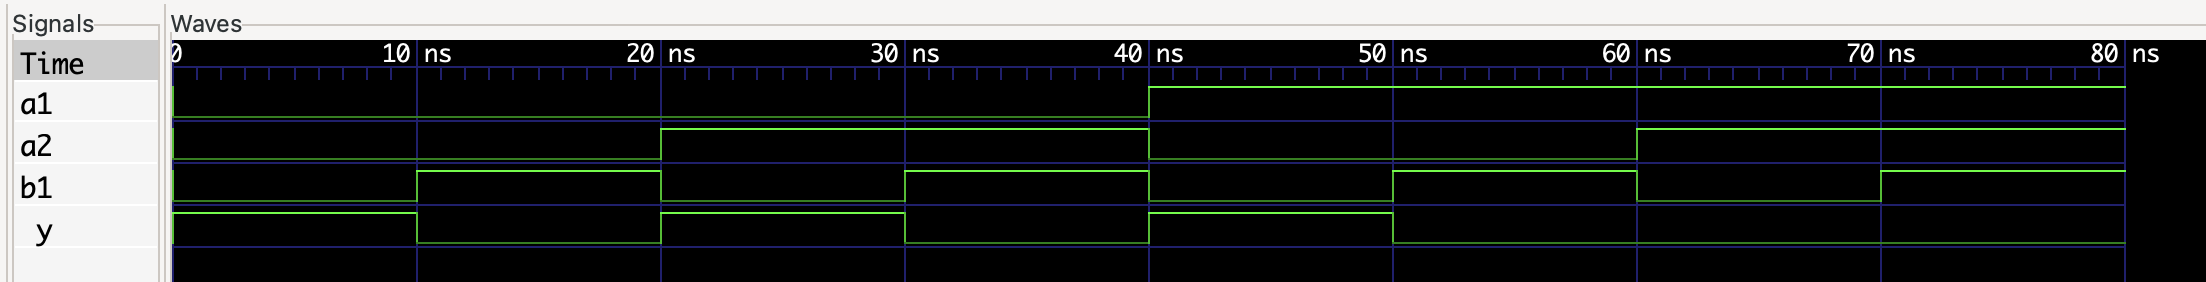
\includegraphics[width=0.8\textwidth]{./a21oi_verilog_result.png}
	\caption{Verilog simulation waveform of the a21oi cell}
	\label{fig:a21oi_verilog_waveform}
\end{figure}

\clearpage

\section{Cell: dfxtn}

\subsection{Circuit Diagram}
Figure~\ref{fig:dff_circuit} shows the schematic of the dfxtn cell.
\begin{figure}[H]
	\centering
	\includegraphics[width=0.7\textwidth]{./dff.eps}
	\caption{Circuit diagram of the dfxtn cell}
	\label{fig:dff_circuit}
\end{figure}

\subsection{Transistor Dimensions}
The width and length of the MOSFETs used in the cell are listed in Table~\ref{tab:mosfet_dims}.

\begin{table}[H]
	\centering
	\begin{tabular}{|c|c|c|}
		\hline
		     & \textbf{Width ($\mu$m)} & \textbf{Length ($\mu$m)} \\
		\hline
		PMOS & 1.26                    & 0.15                     \\
		NMOS & 0.42                    & 0.15                     \\
		\hline
	\end{tabular}
	\caption{MOSFET width and length values for the dfxtn cell}
	\label{tab:mosfet_dims}
\end{table}

\subsection{Layout}
The layout of the dfxtn cell is shown in Figure~\ref{fig:dff_layout}. The cell area is measured as:
\[
	\text{Area} = 31.95 \mu \times 2.72 \mu = 86.904 \mu m^2
\]

\begin{figure}[H]
	\centering
	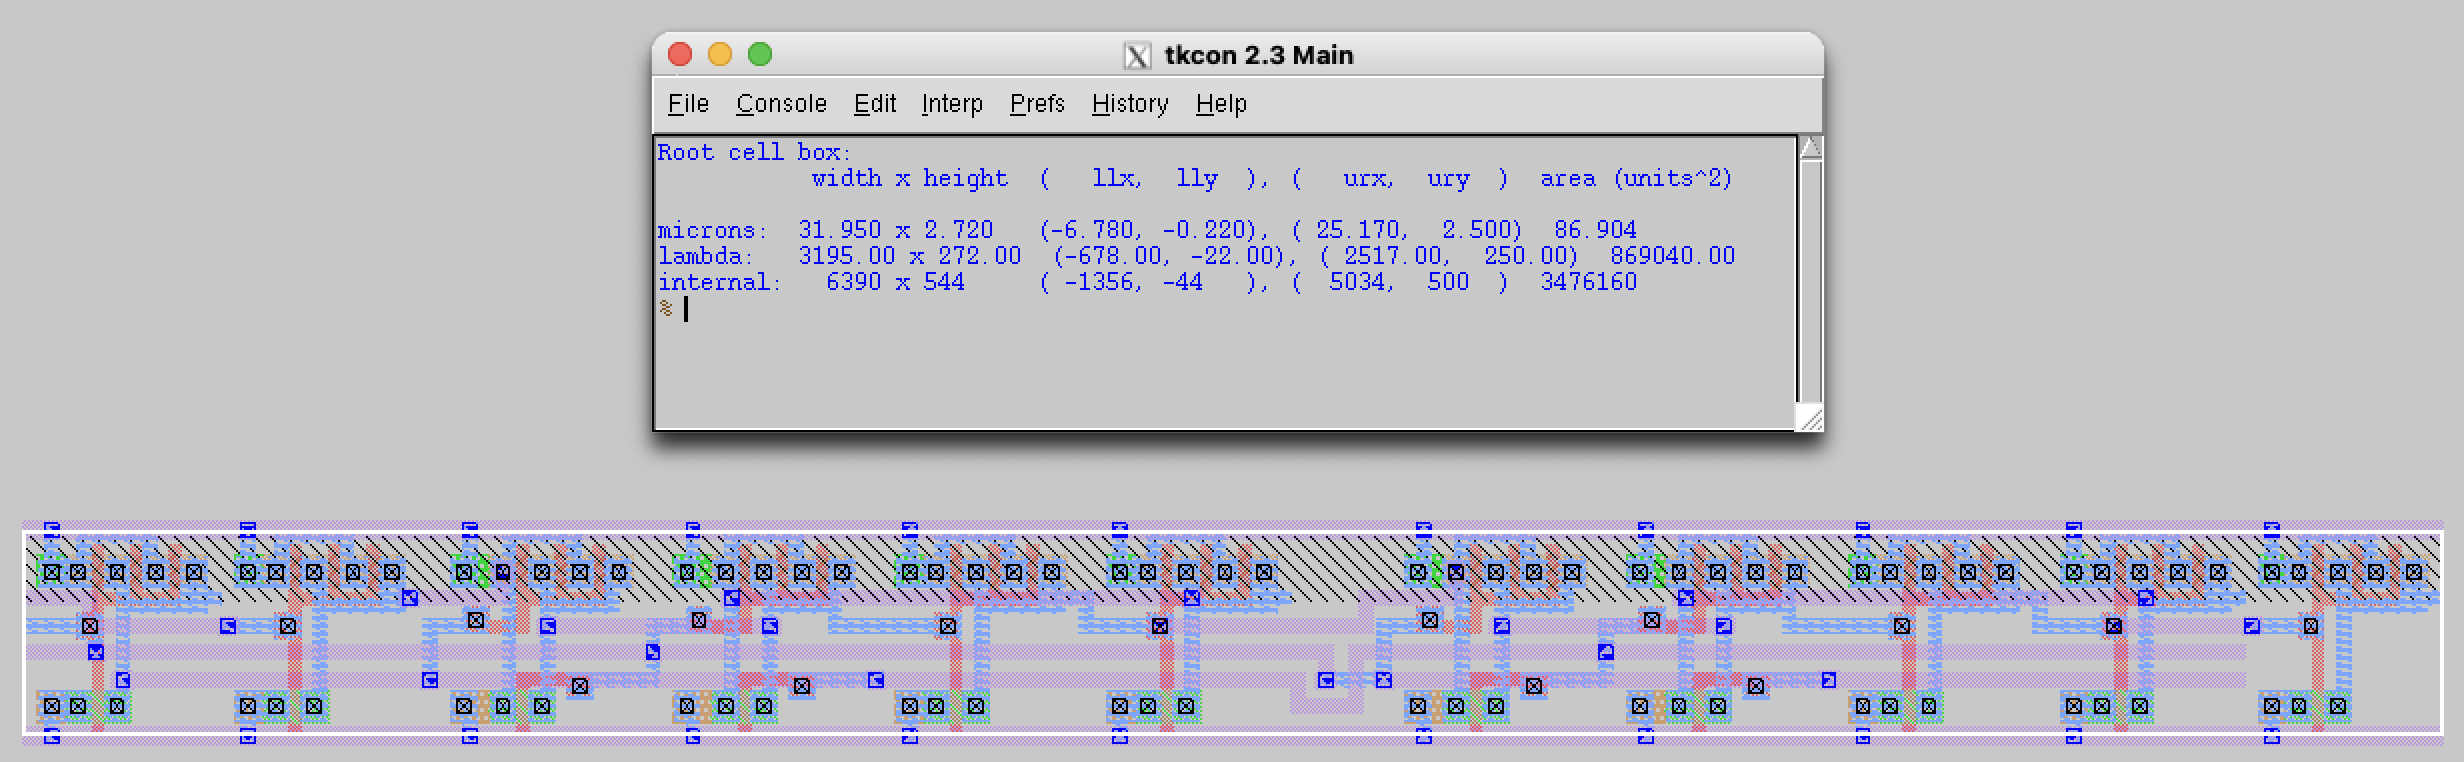
\includegraphics[width=0.7\textwidth]{./dff_layout.png}
	\caption{Layout of the dfxtn cell}
	\label{fig:dff_layout}
\end{figure}

\subsection{Original Netlist}
The netlist written for the dfxtn cell is shown below:
\lstinputlisting[language={}]{../dfxtn/ngspice_simulations/dfxtn_schematic.spice}

\subsection{PEX Netlist}
The extracted netlist of the cell is shown below:
\lstinputlisting[language={}]{../dfxtn/ngspice_simulations/dfxtn_layout_pex.spice}

\clearpage

\subsection{Verification}
The DRC and LVS results are clean (Figure~\ref{fig:dff_verification}).

\begin{figure}[H]
	\centering
	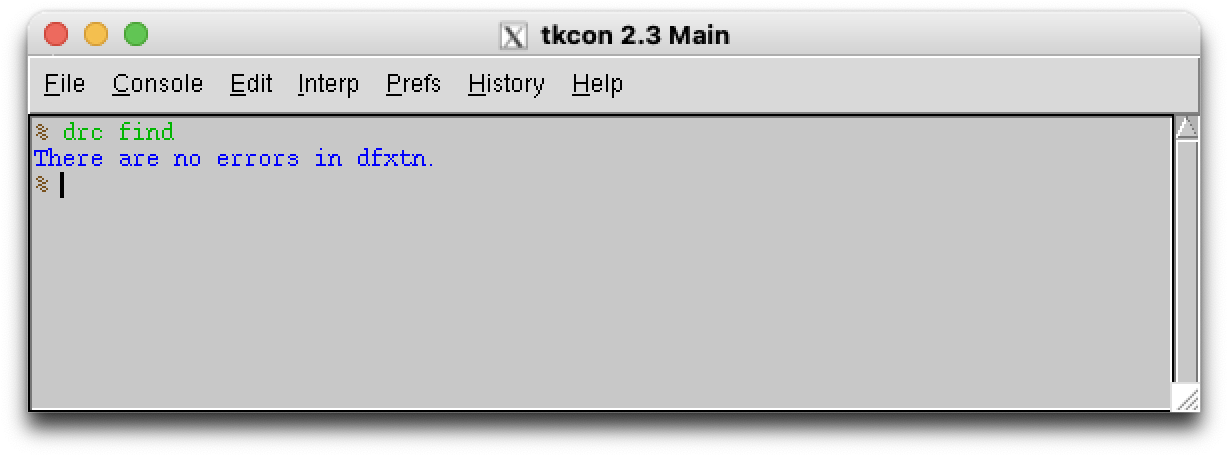
\includegraphics[width=0.45\textwidth]{./dfxtn_drc.png}
	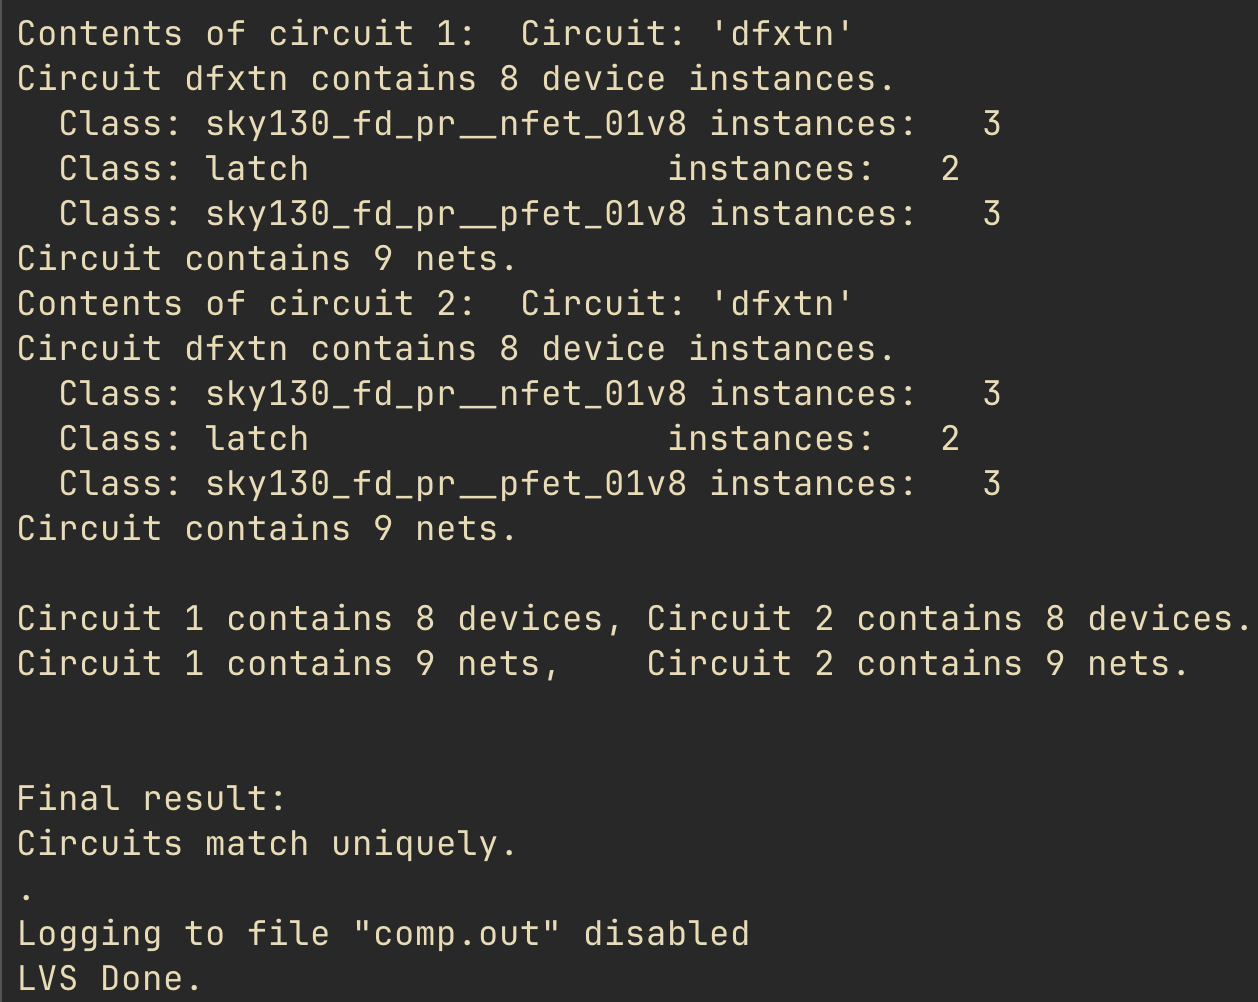
\includegraphics[width=0.45\textwidth]{./lvs_dfxtn.png}
	\caption{DRC and LVS clean results for the DFF cell}
	\label{fig:dff_verification}
\end{figure}


\subsection{Waveforms}
Waveforms from simulations showing input, output, and clock signals for rise and fall transitions, propagation delay, set-up time, and hold time are shown below. Each timing metric has separate plots for rise and fall transitions.

\begin{figure}[H]
	\centering
	% Propagation delay
	\begin{subfigure}[b]{0.45\textwidth}
		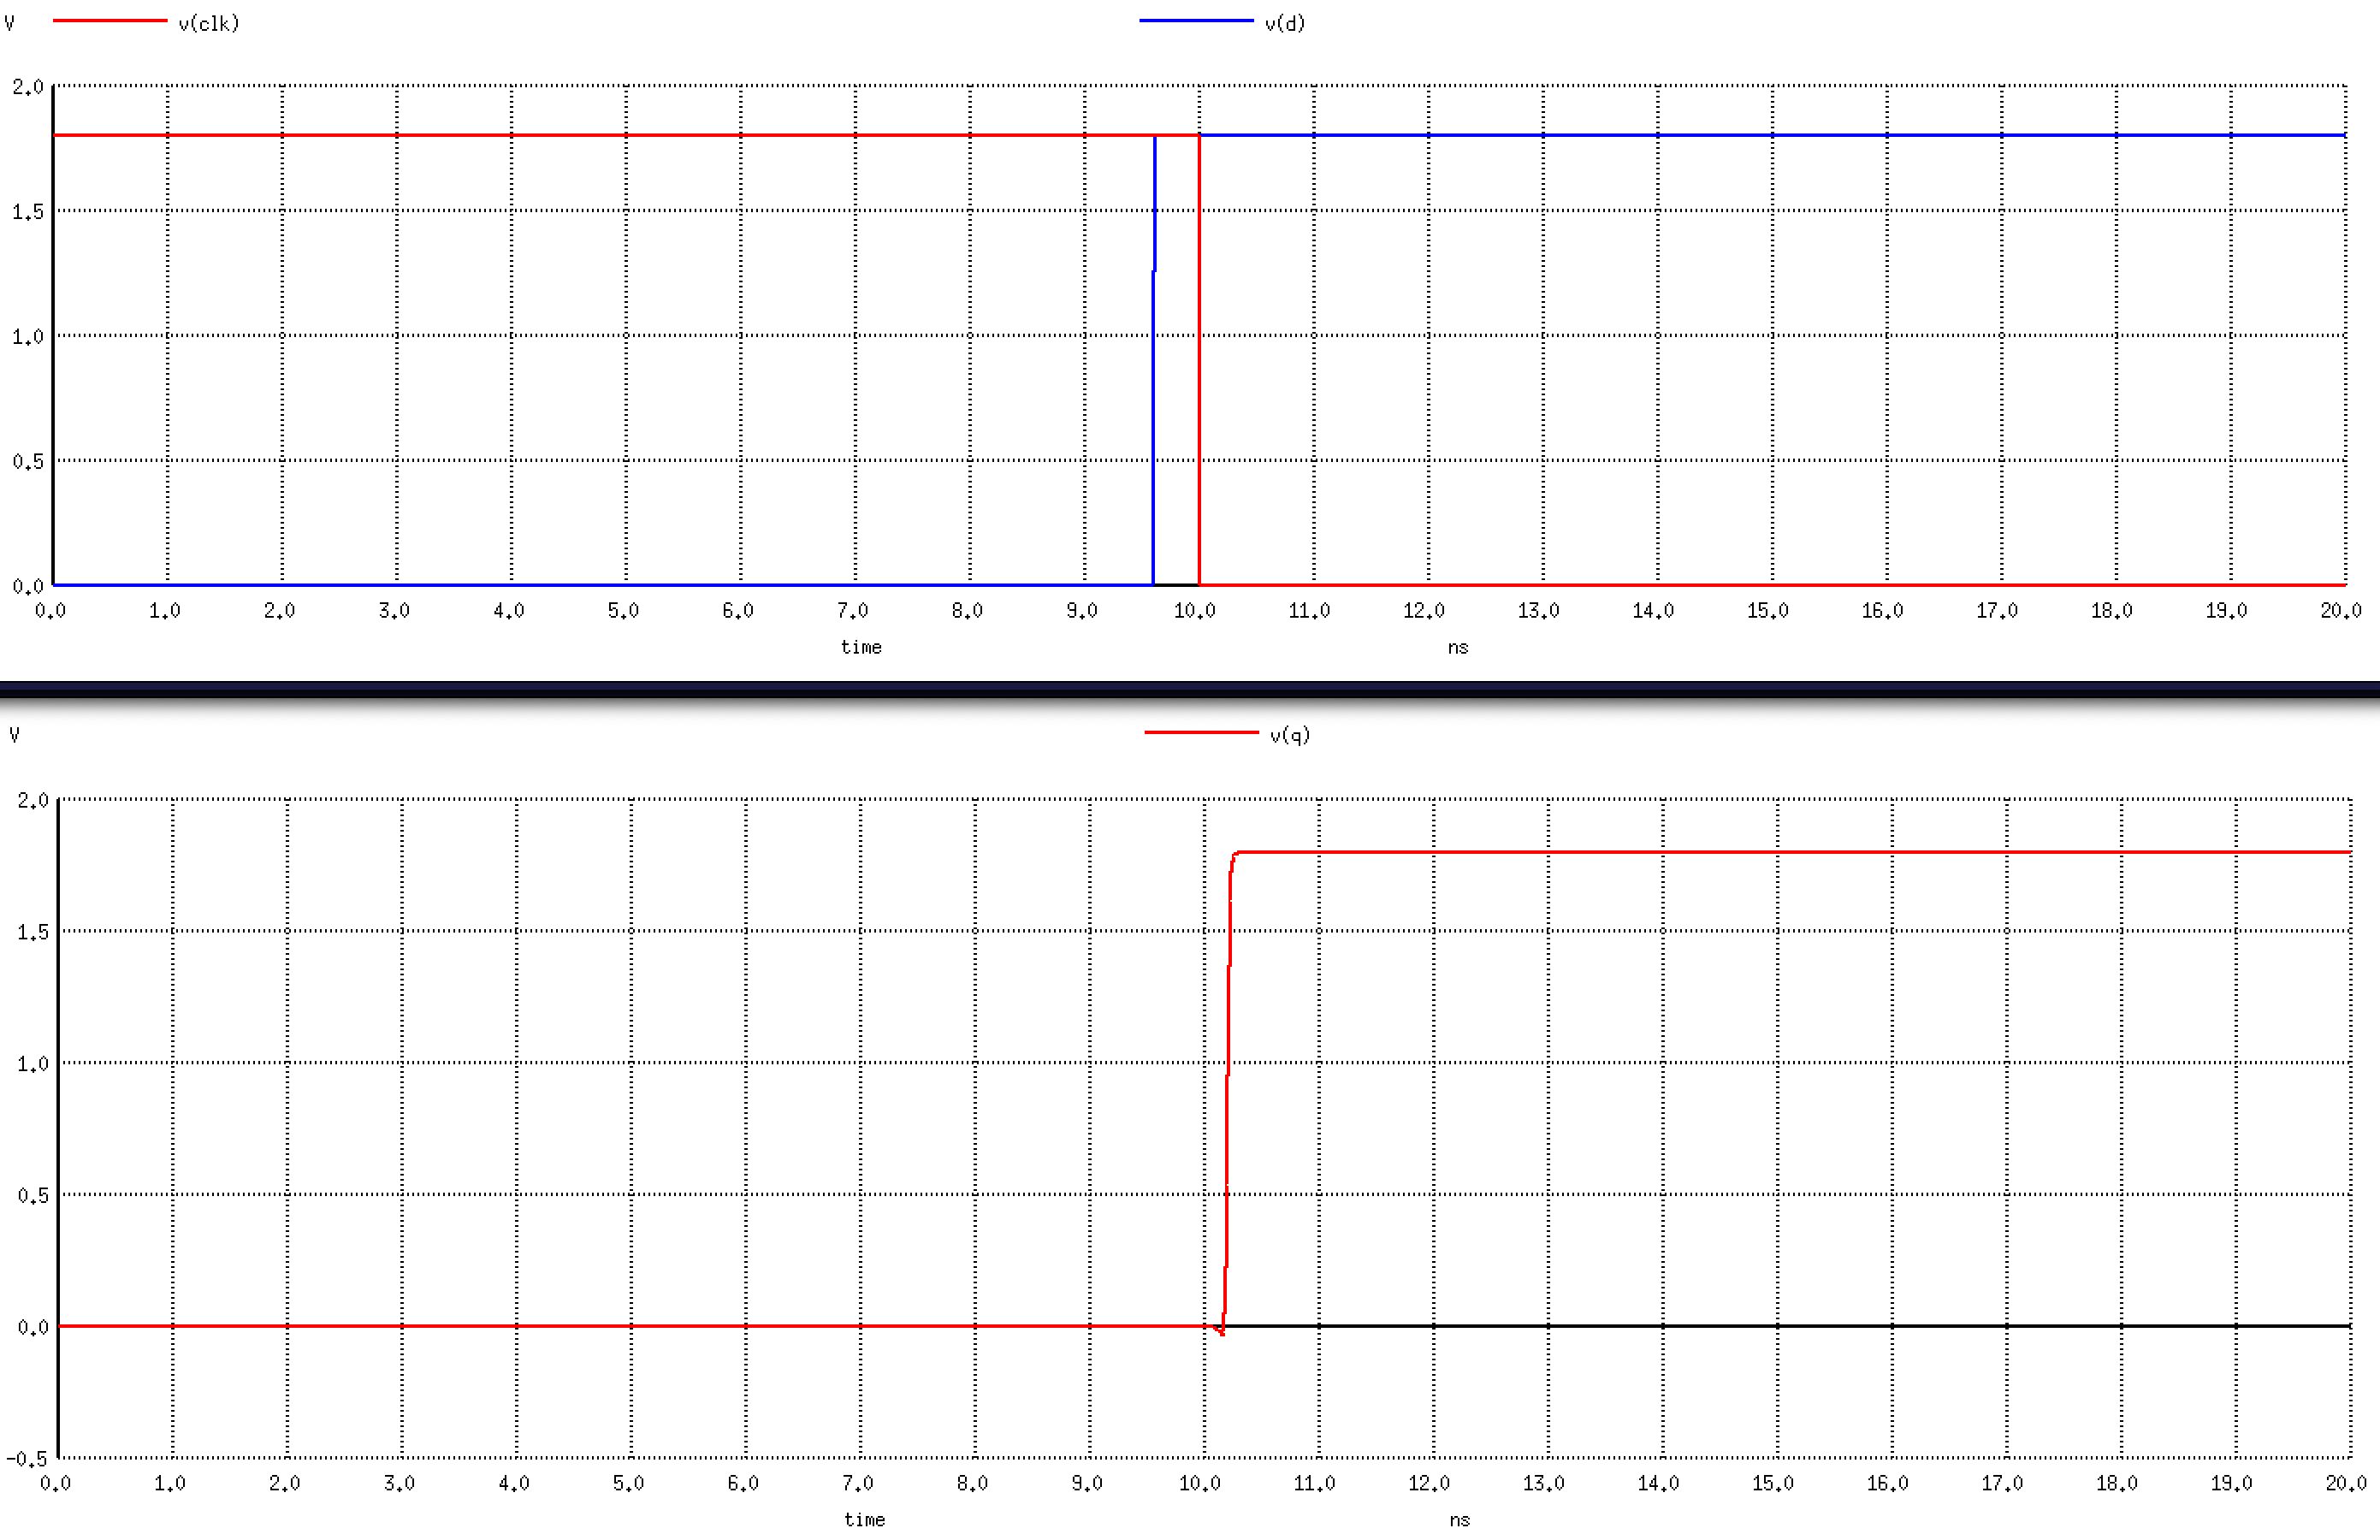
\includegraphics[width=\textwidth]{../dfxtn/ngspice_simulations/images/tcq_c0.5_d10_rise.png}
		\caption{Propagation delay rise ($t_{cq}$)}
		\label{fig:tcq_rise}
	\end{subfigure}
	\hfill
	\begin{subfigure}[b]{0.45\textwidth}
		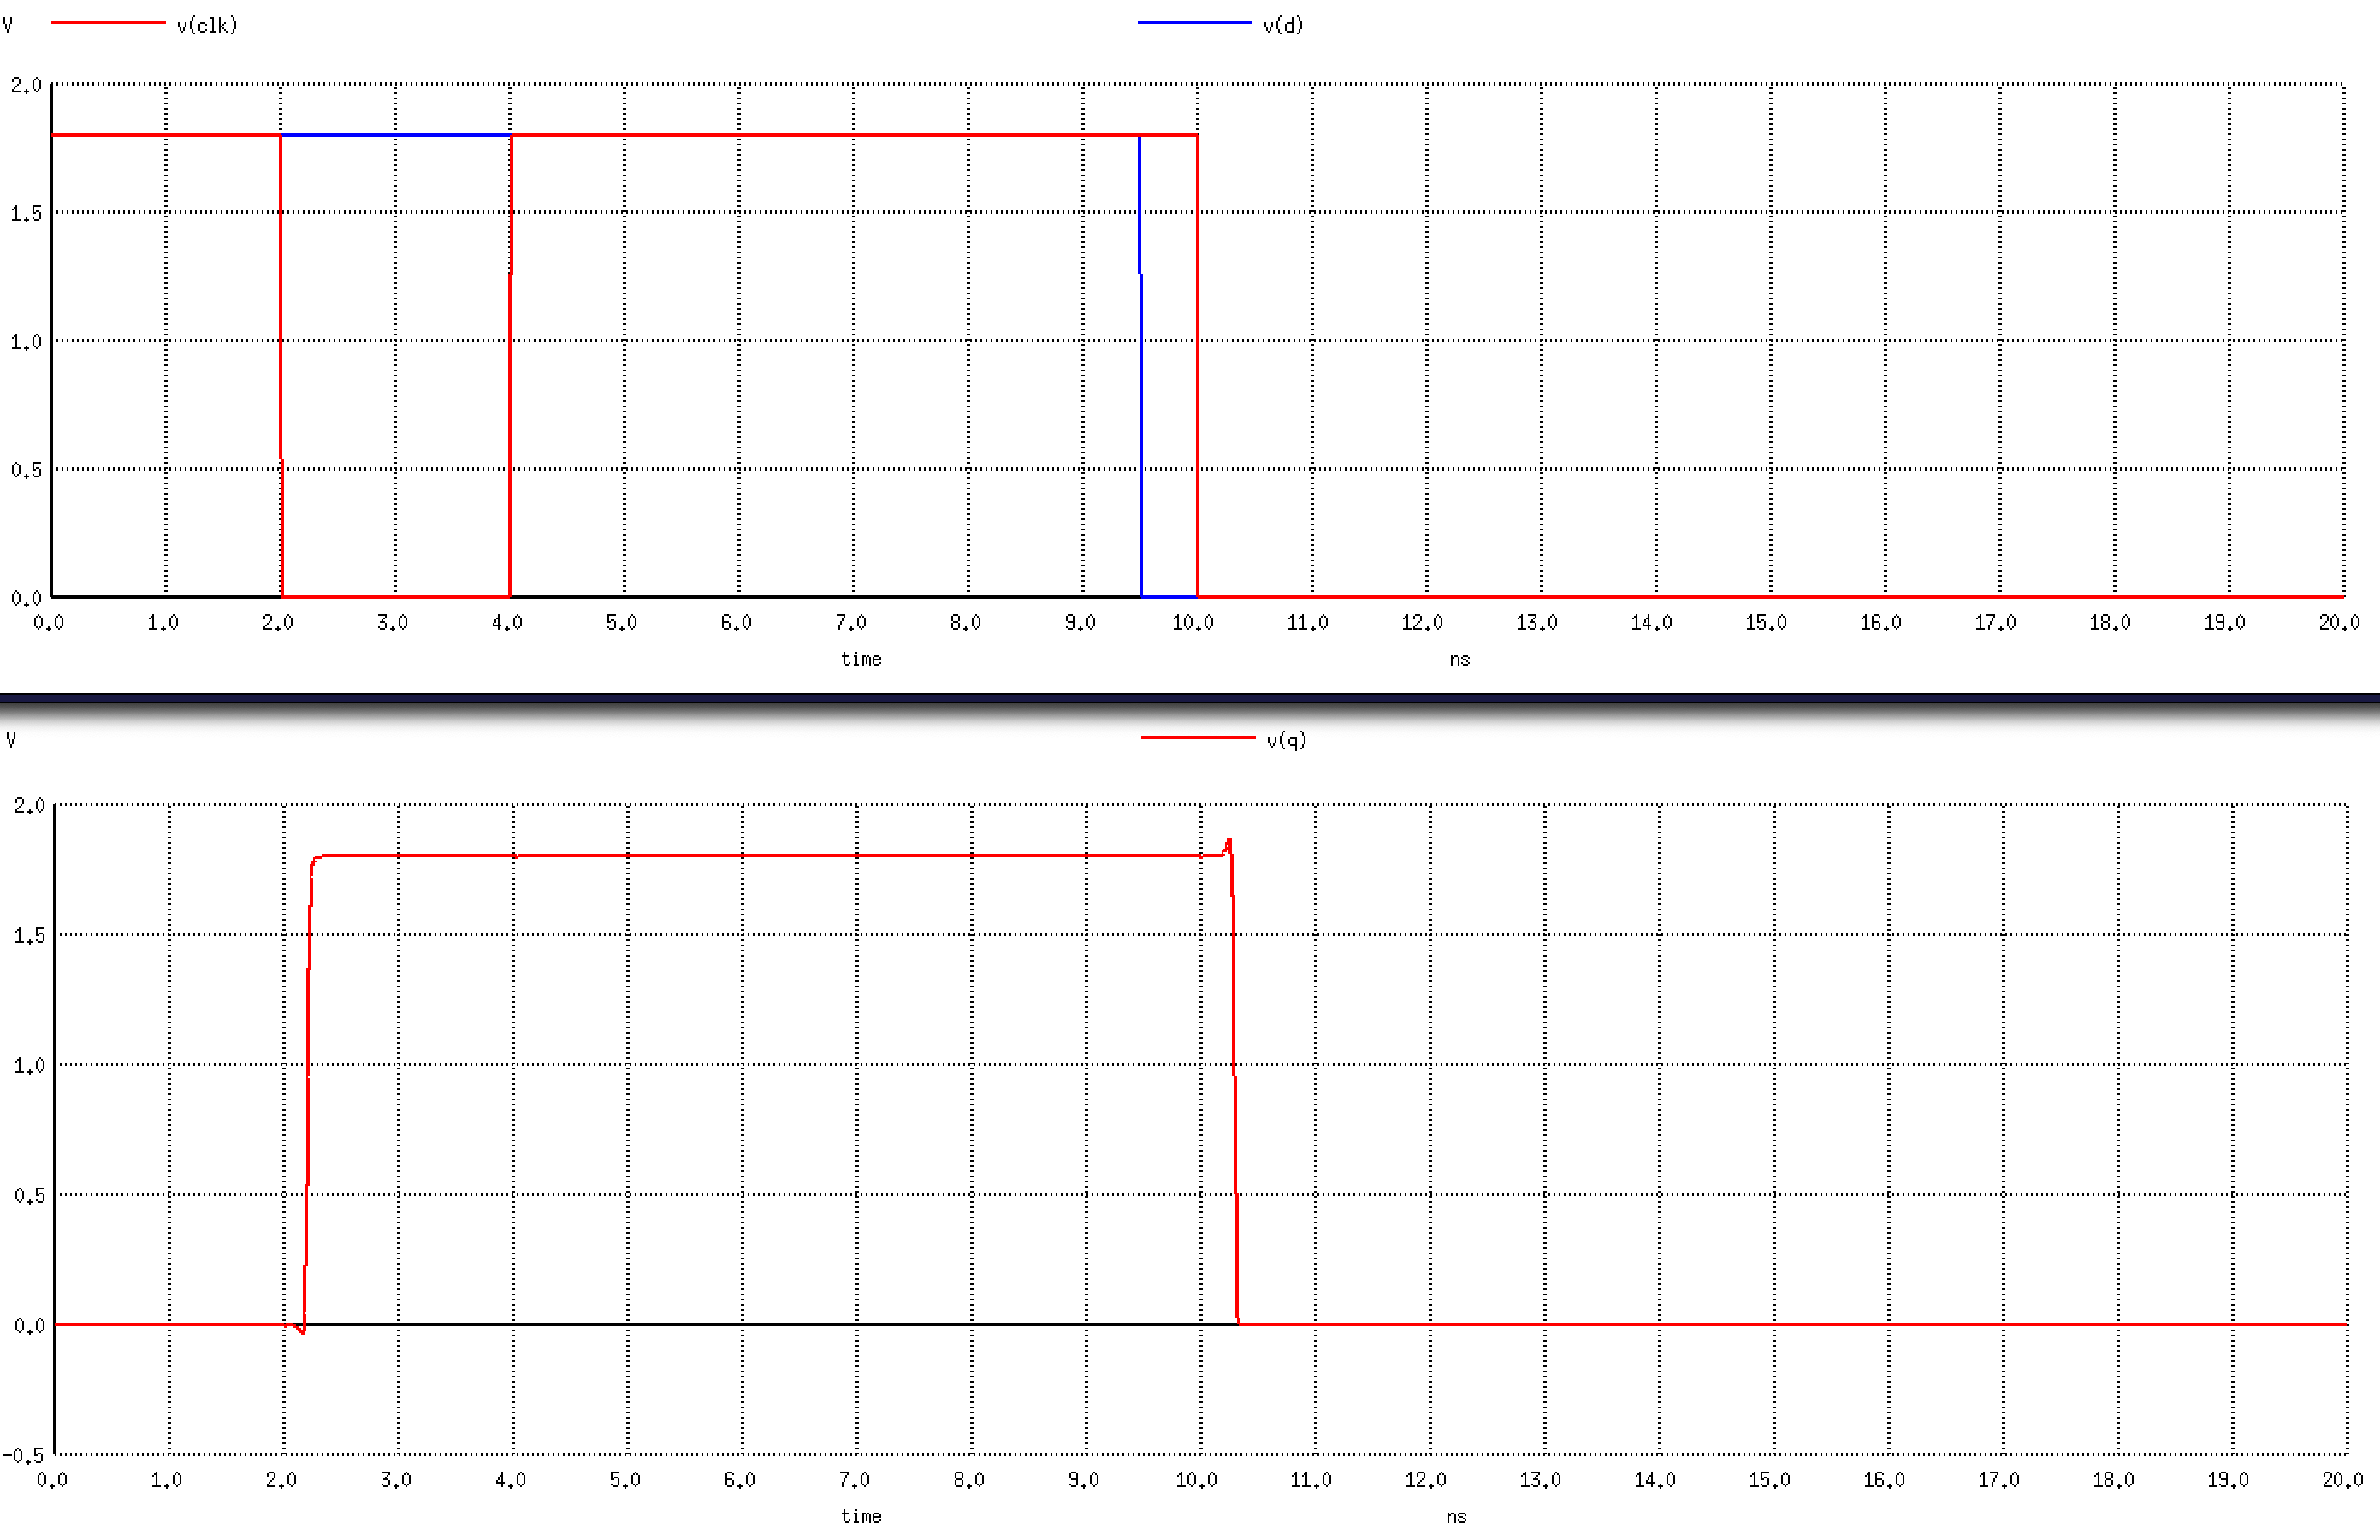
\includegraphics[width=\textwidth]{../dfxtn/ngspice_simulations/images/tcq_c0.5_d10_fall.png}
		\caption{Propagation delay fall ($t_{cq}$)}
		\label{fig:tcq_fall}
	\end{subfigure}

	\vspace{0.5em}

	% Transition times
	\begin{subfigure}[b]{0.45\textwidth}
		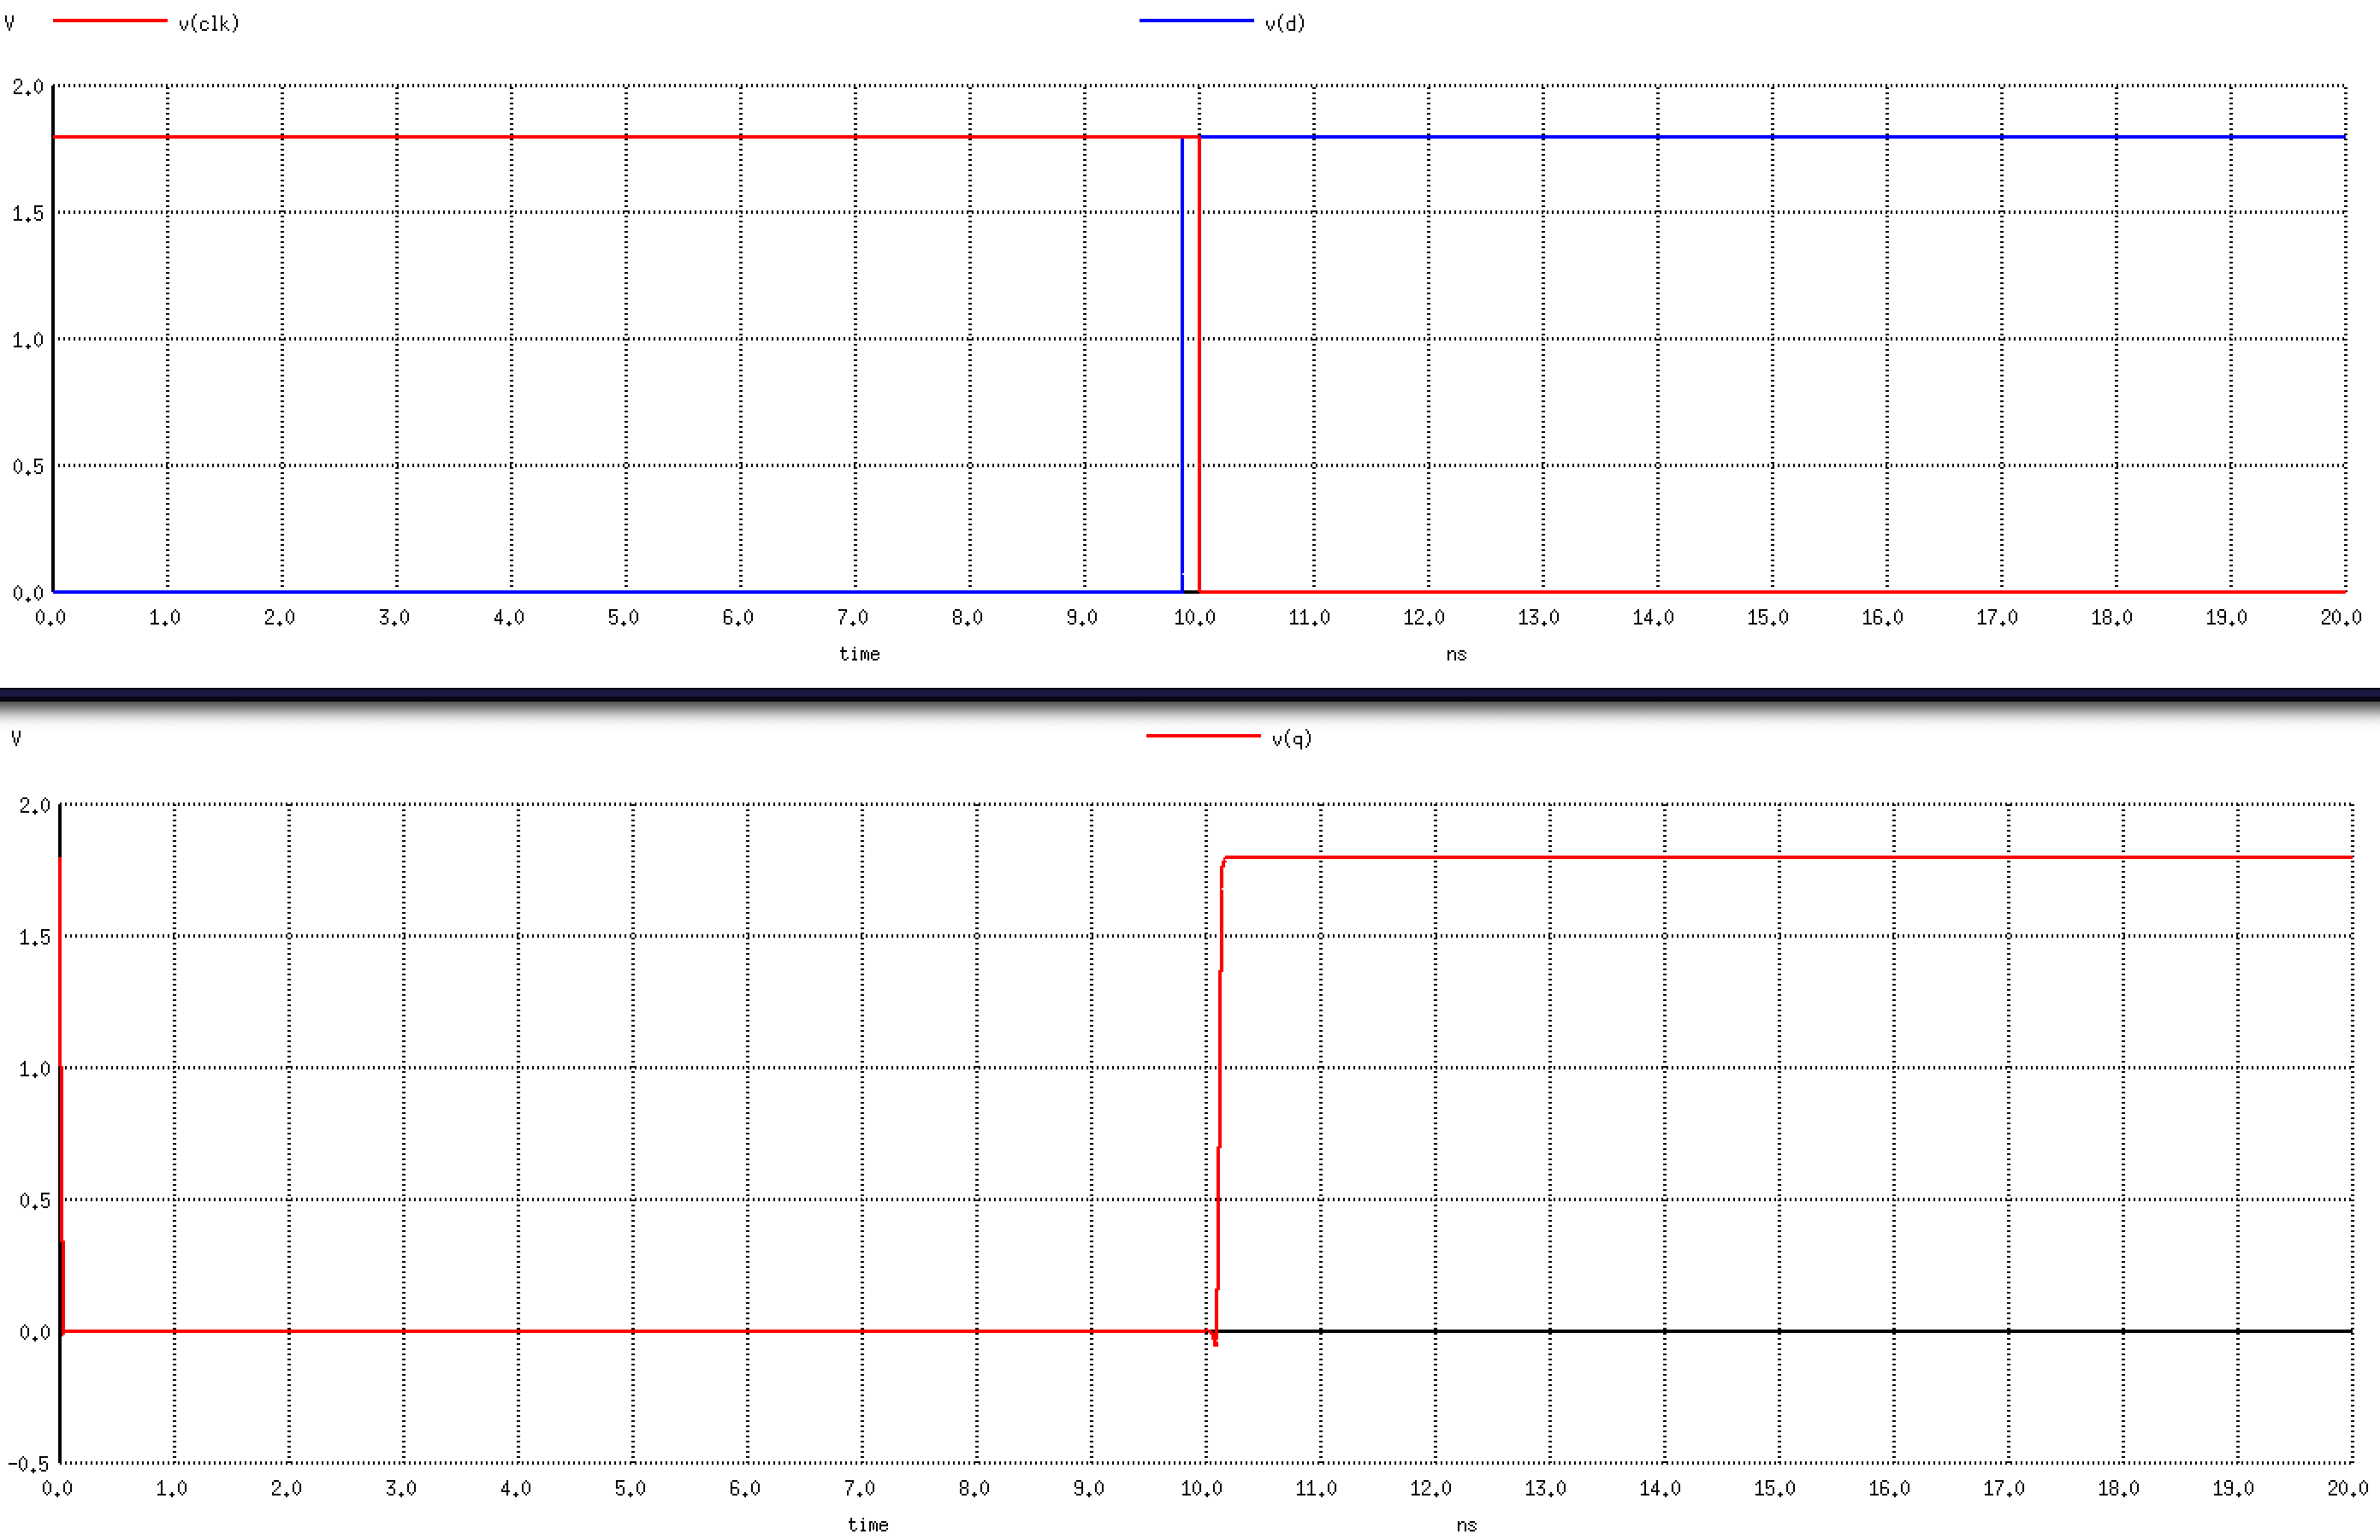
\includegraphics[width=\textwidth]{../dfxtn/ngspice_simulations/images/transition_time_c0.5_d10.png}
		\caption{Rise transition time ($t_{rise}$)}
		\label{fig:trise}
	\end{subfigure}
	\hfill
	\begin{subfigure}[b]{0.45\textwidth}
		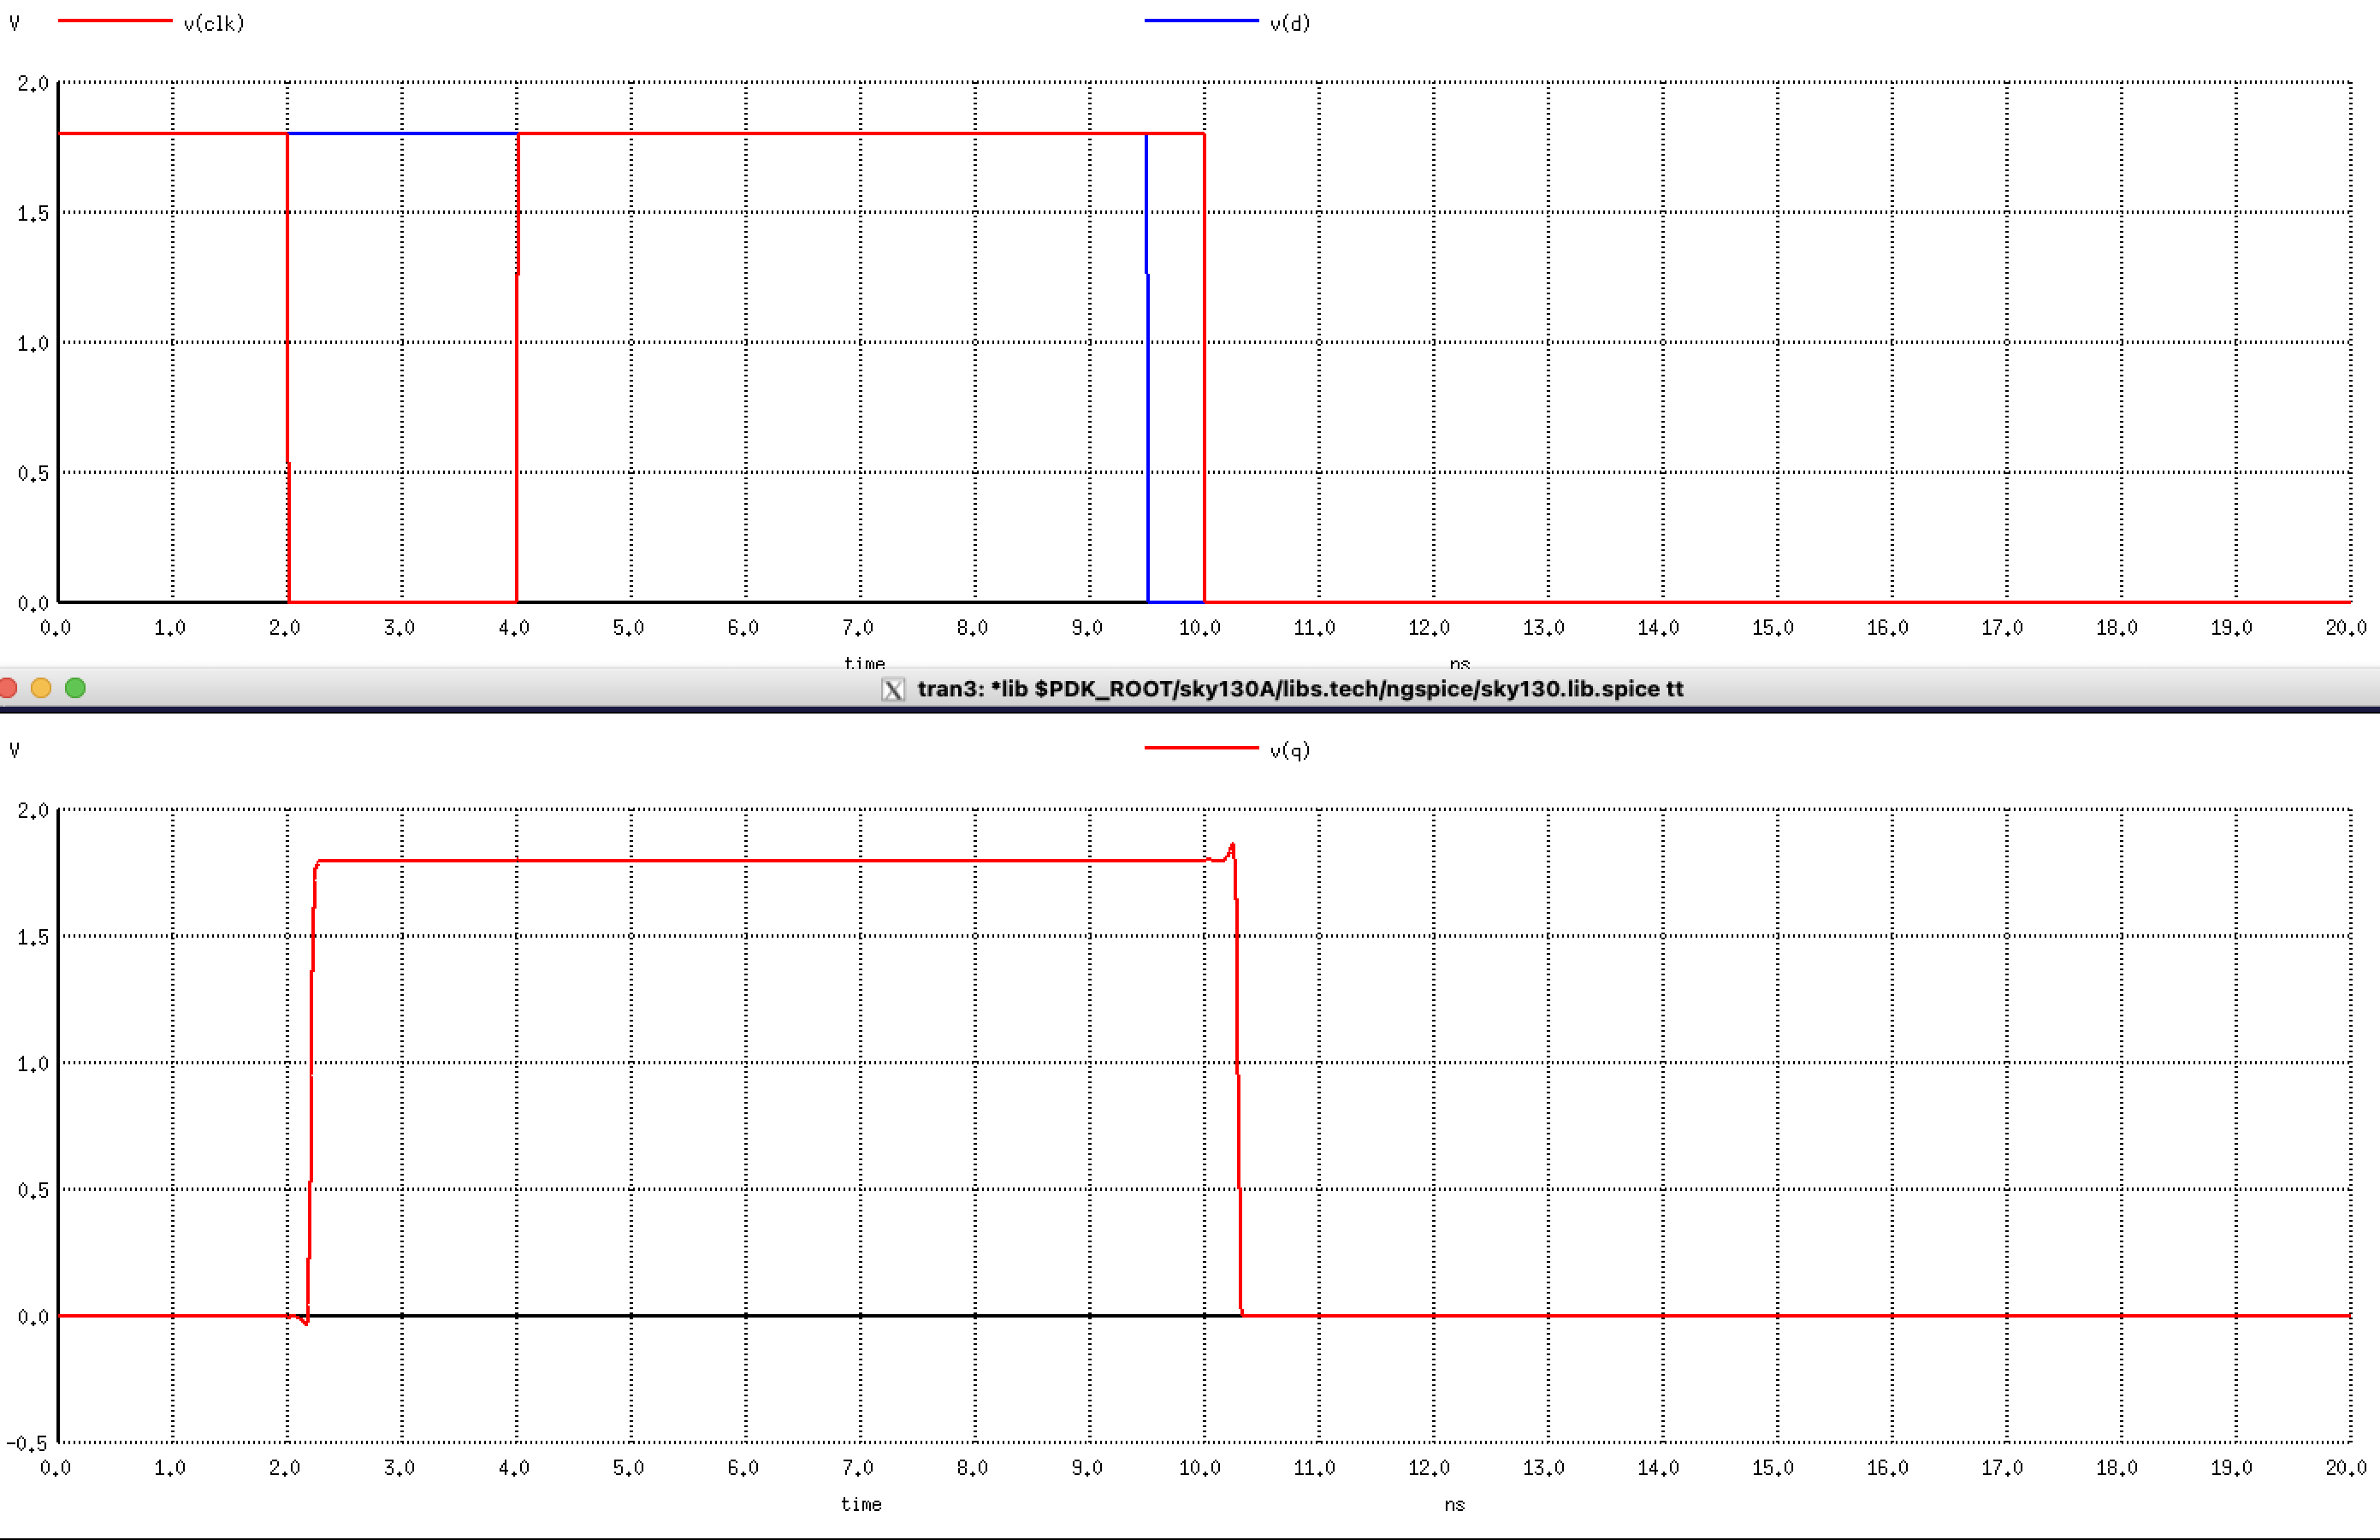
\includegraphics[width=\textwidth]{../dfxtn/ngspice_simulations/images/transition_time_c0.5_d10_fall.png}
		\caption{Fall transition time ($t_{fall}$)}
		\label{fig:tfall}
	\end{subfigure}

	\vspace{0.5em}

	% Set-up time
	\begin{subfigure}[b]{0.45\textwidth}
		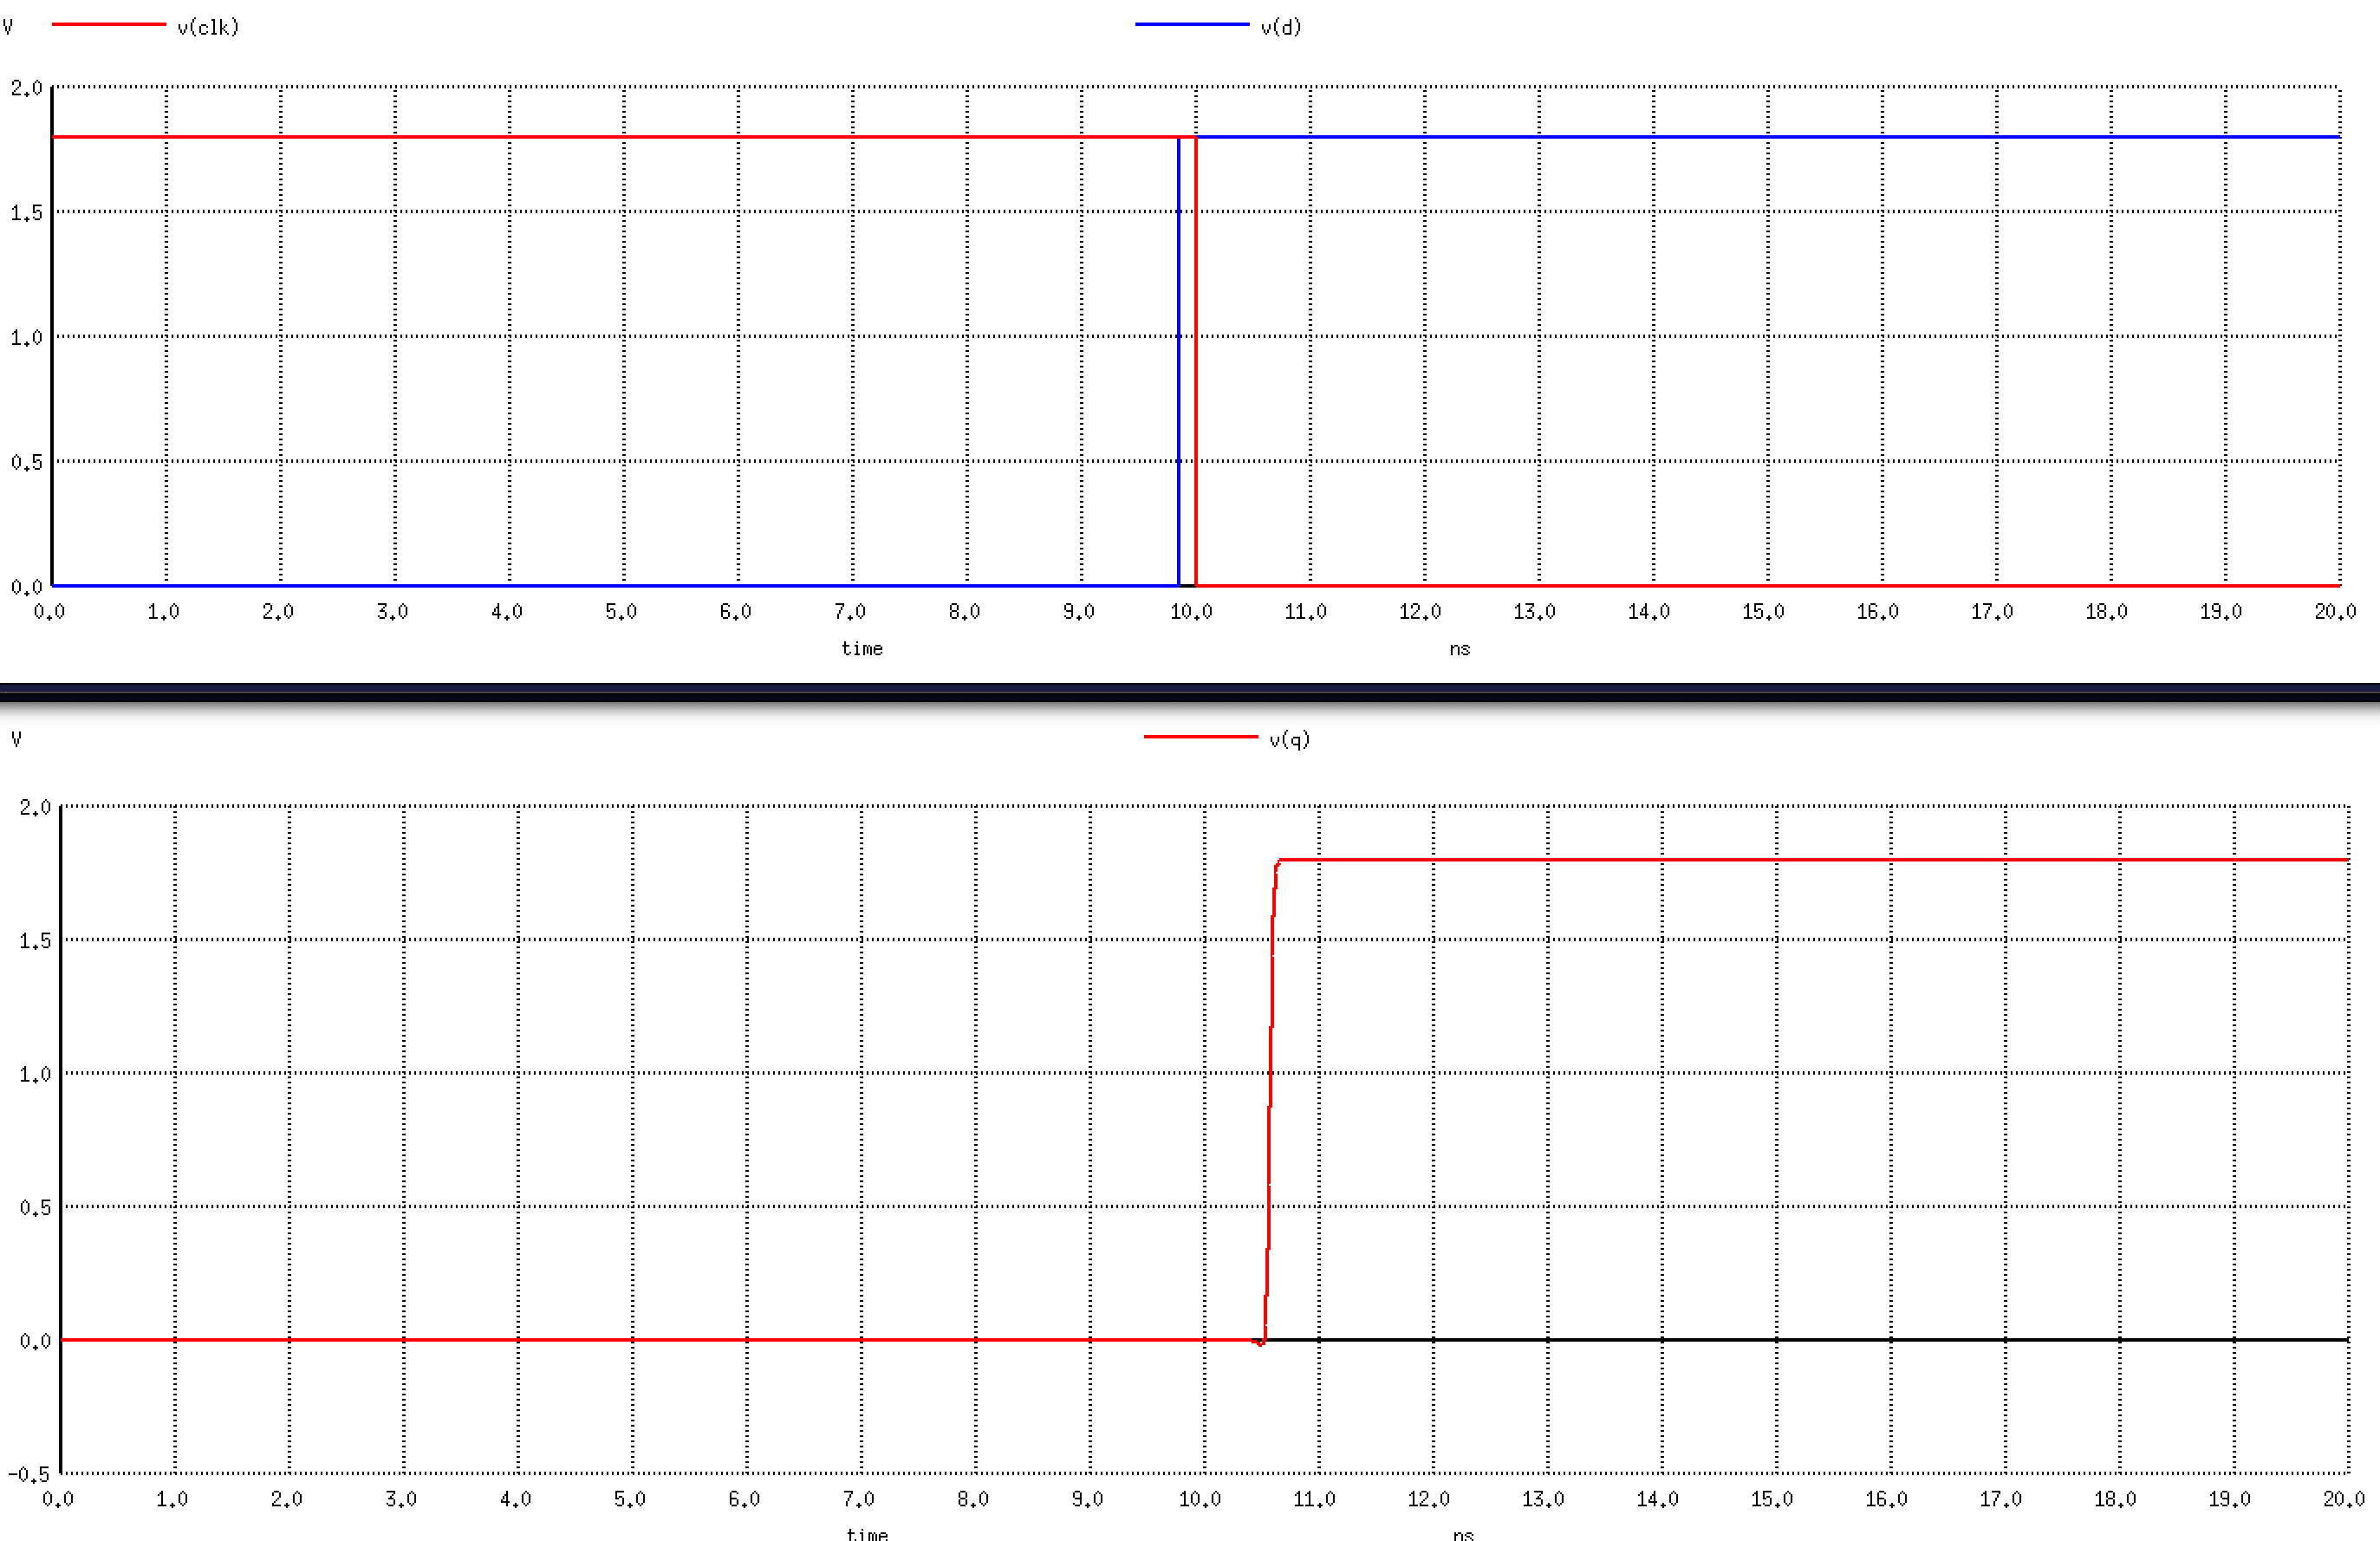
\includegraphics[width=\textwidth]{../dfxtn/ngspice_simulations/images/tsu_d10_clk10_rise.png}
		\caption{Set-up time rise ($t_{setup}$)}
		\label{fig:tsetup_rise}
	\end{subfigure}
	\hfill
	\begin{subfigure}[b]{0.45\textwidth}
		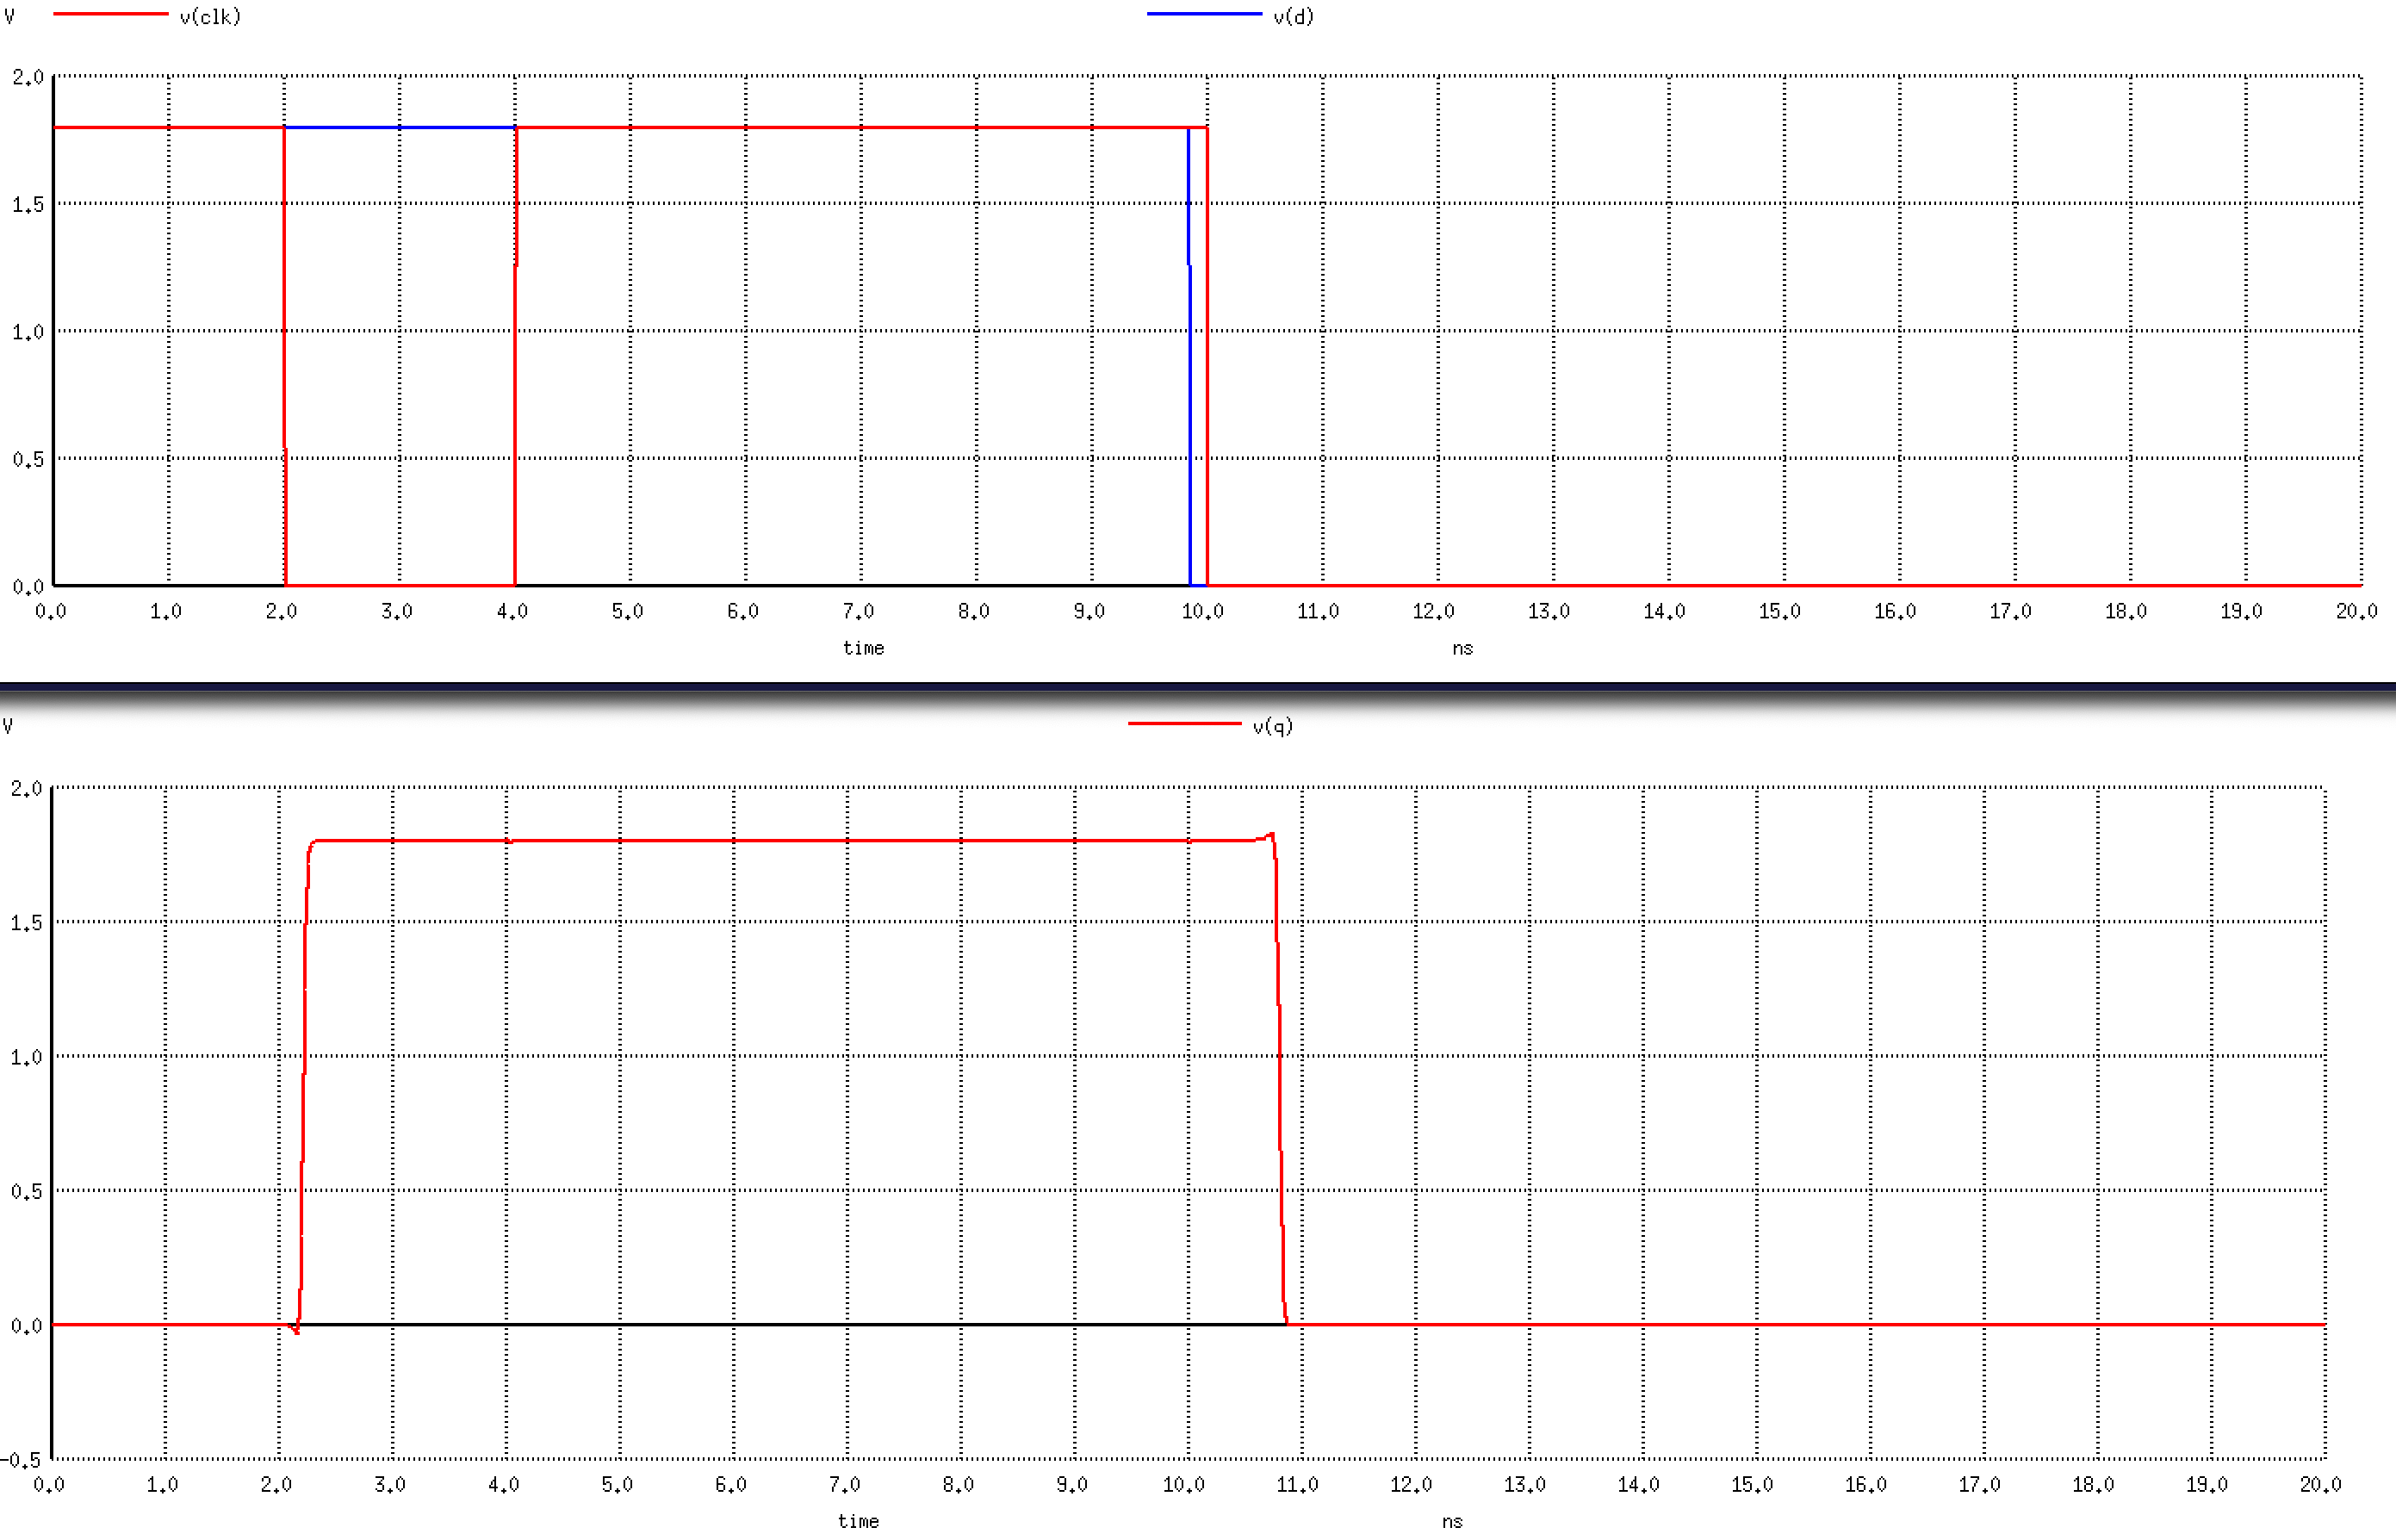
\includegraphics[width=\textwidth]{../dfxtn/ngspice_simulations/images/tsu_d10_clk10_fall.png}
		\caption{Set-up time fall ($t_{setup}$)}
		\label{fig:tsetup_fall}
	\end{subfigure}

	\vspace{0.5em}

	% Hold time
	\begin{subfigure}[b]{0.45\textwidth}
		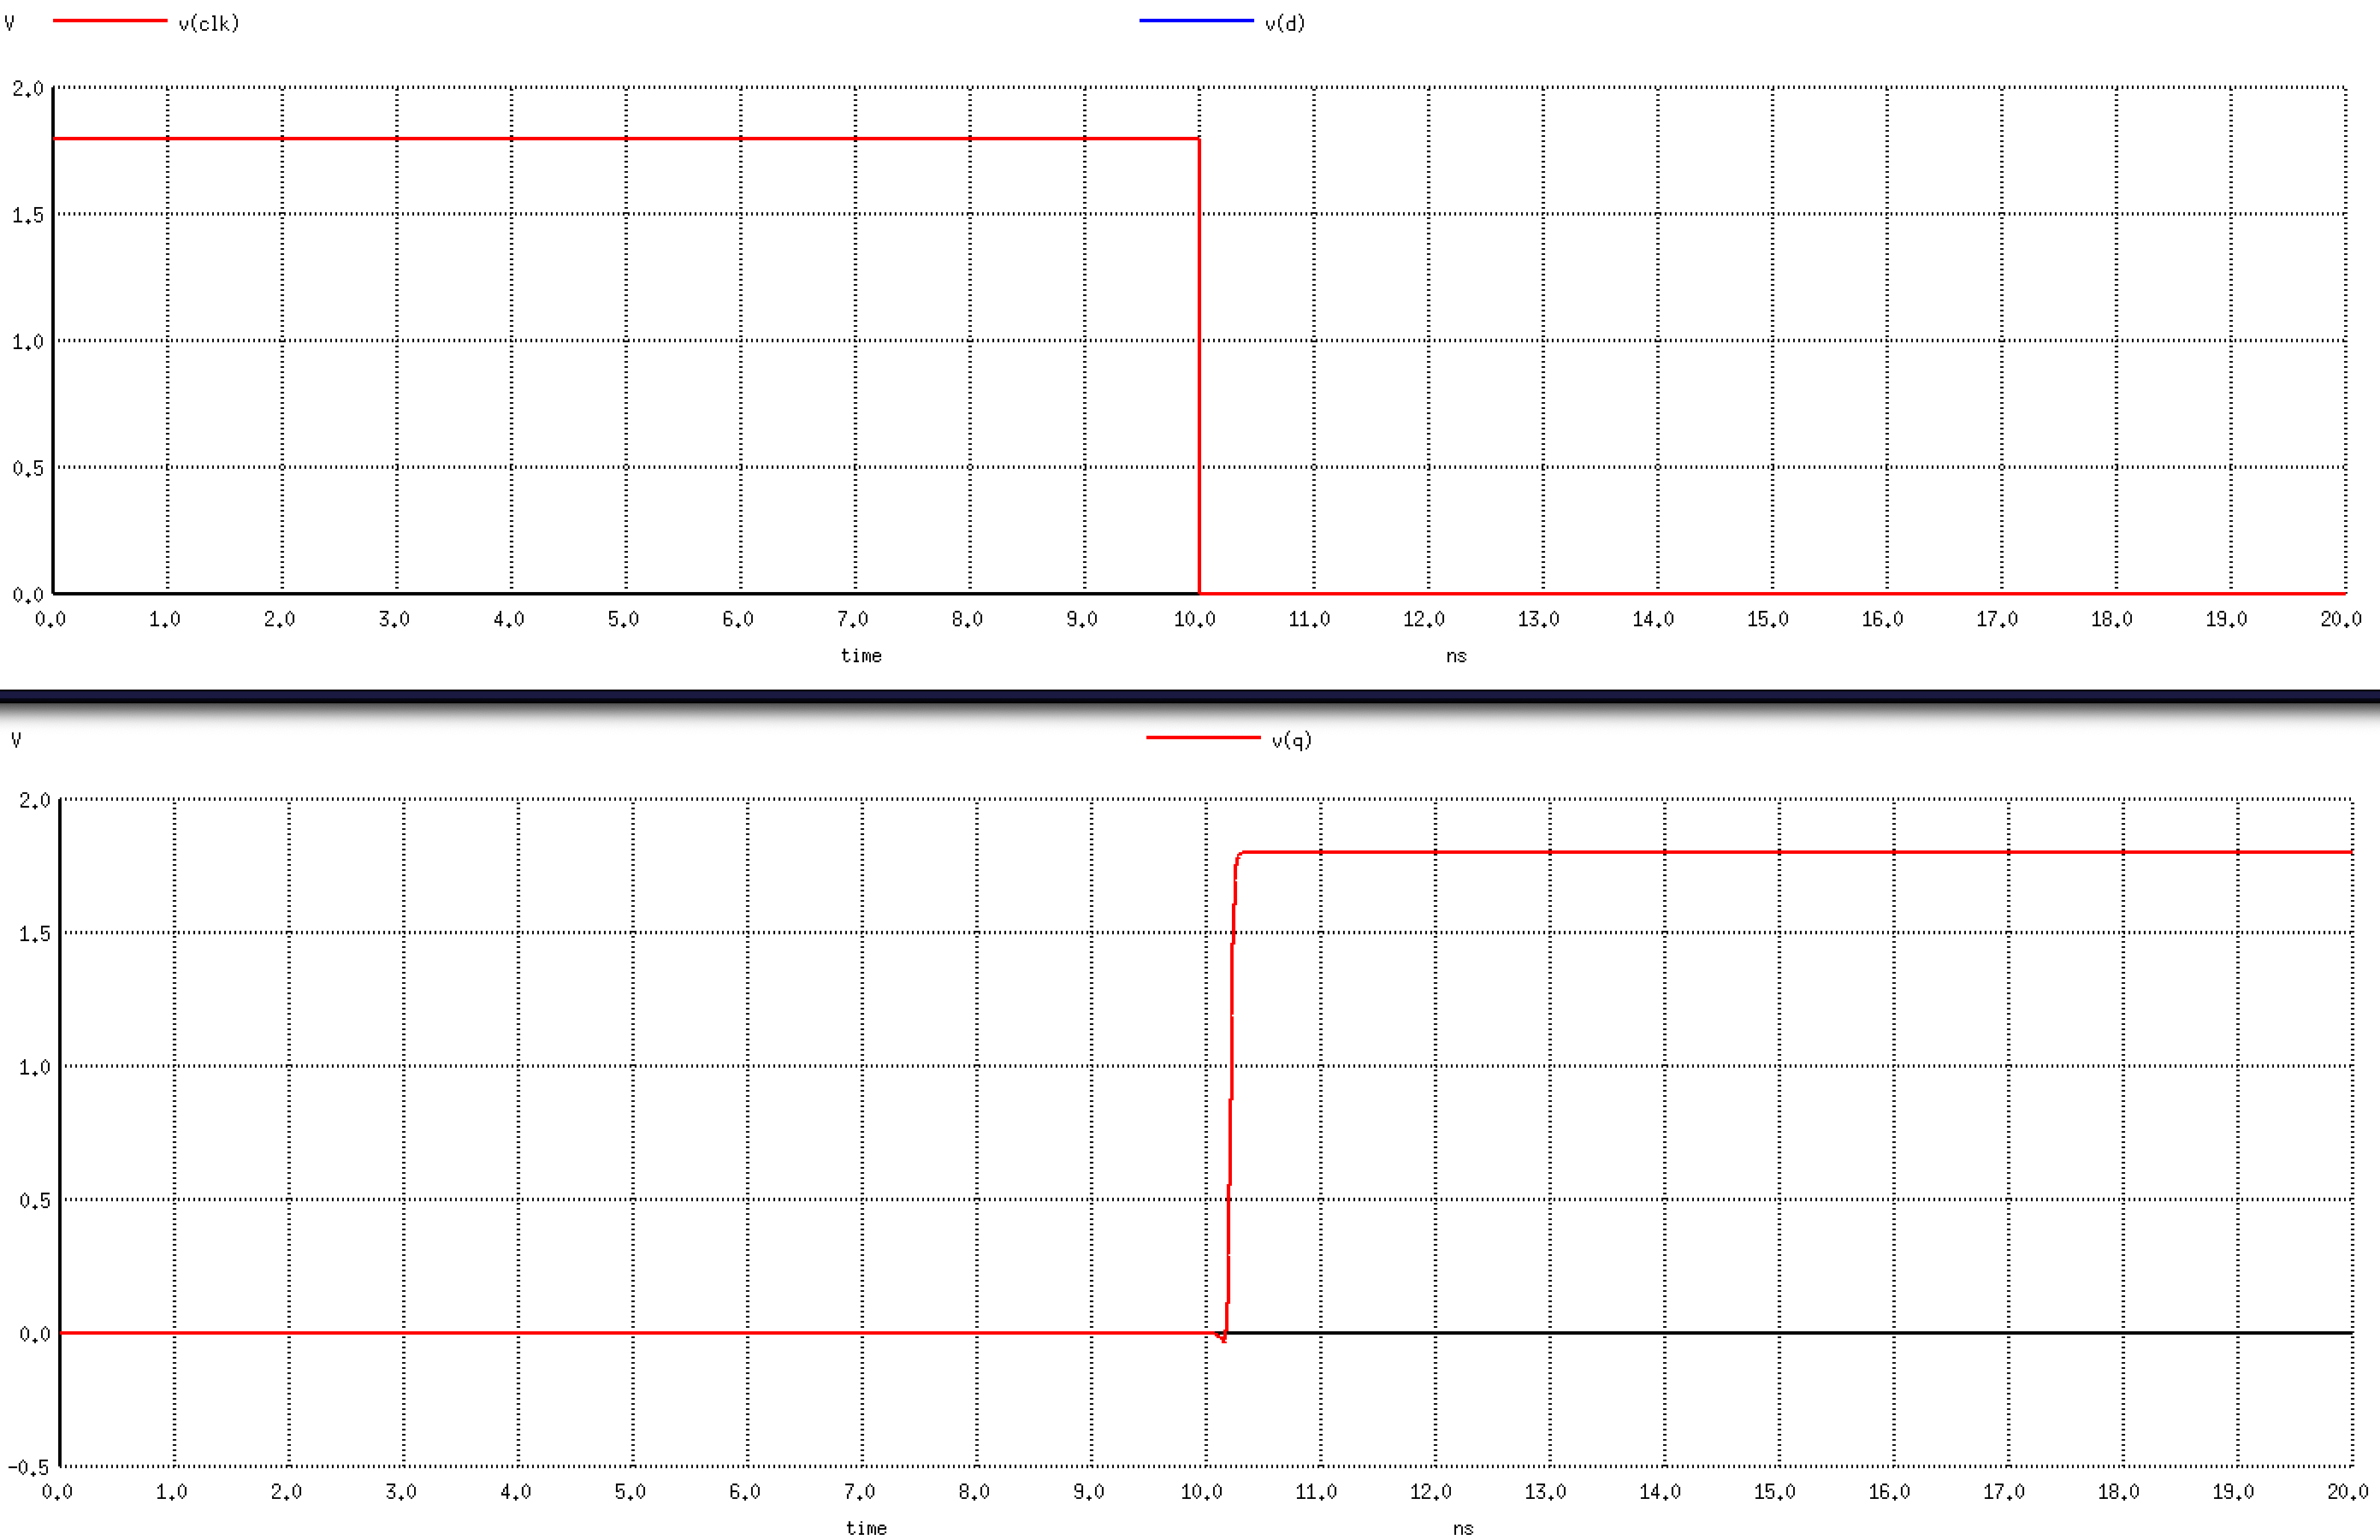
\includegraphics[width=\textwidth]{../dfxtn/ngspice_simulations/images/thold_d10_clk10_rise.png}
		\caption{Hold time rise ($t_{hold}$)}
		\label{fig:thold_rise}
	\end{subfigure}
	\hfill
	\begin{subfigure}[b]{0.45\textwidth}
		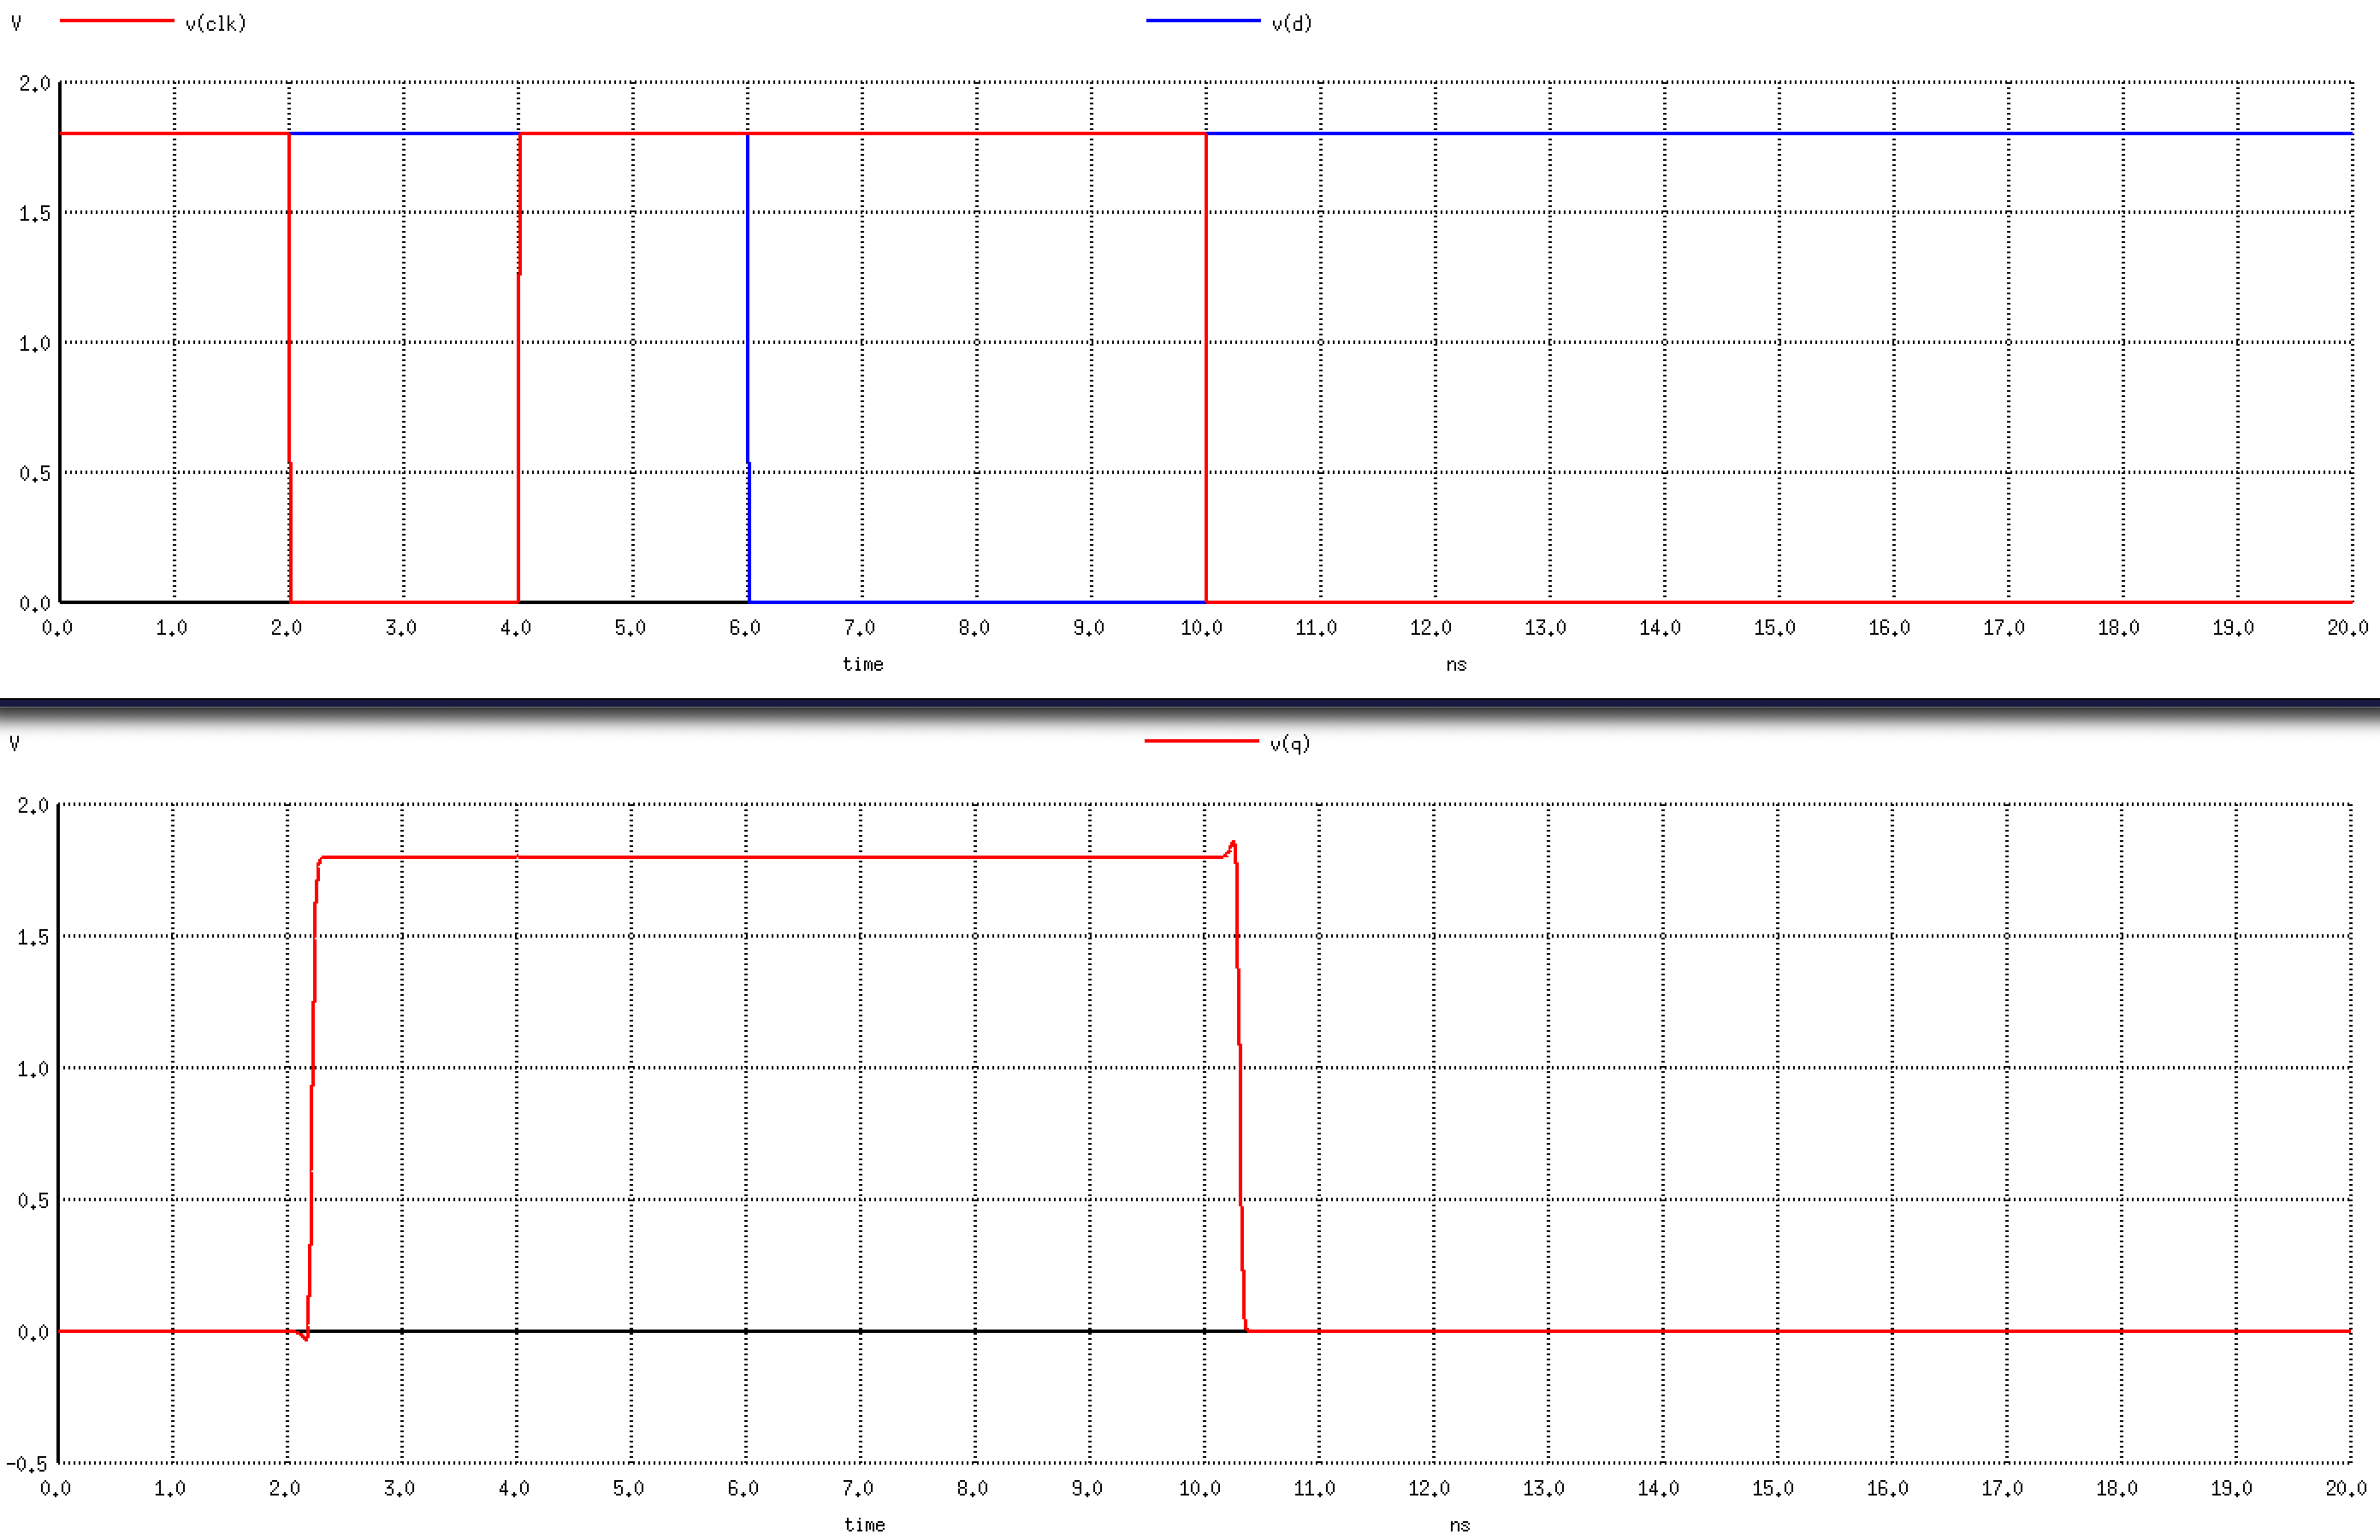
\includegraphics[width=\textwidth]{../dfxtn/ngspice_simulations/images/thold_d10_clk10_fall.png}
		\caption{Hold time fall ($t_{hold}$)}
		\label{fig:thold_fall}
	\end{subfigure}

	\caption{Waveforms of the DFF cell for rise and fall transitions and timing parameters}
	\label{fig:dff_waveforms}
\end{figure}

\subsection{Timing and Power Characterisation}

% =========================
% Input Pin Capacitances
% =========================
\subsubsection{Input Pin Capacitances}
\begin{table}[H]
	\centering
	\begin{tabular}{|c|c|c|c|}
		\hline
		Input Pins & Rise Cap (fF) & Fall Cap (fF) & Average Cap (fF) \\ \hline
		D          & 4.01855       & 4.01825       & 4.0184           \\ \hline
		CLK        & 20.9715       & 20.9719       & 20.9717          \\ \hline
	\end{tabular}
	\caption{Input pin capacitances}
\end{table}

% =========================
% Setup Time
% =========================
\subsubsection{Set-up Time}

\begin{table}[H]
	\centering
	\begin{tabular}{|c|c|c|}
		\hline
		        & 10 ps & 1000 ps \\ \hline
		10 ps   & 0.152 & 0.333   \\ \hline
		1000 ps & 0.243 & 0.409   \\ \hline
	\end{tabular}
	\caption{Rise Constraint (in ns) [Input slew vs CLK slew]}
\end{table}

\begin{table}[H]
	\centering
	\begin{tabular}{|c|c|c|}
		\hline
		        & 10 ps & 1000 ps \\ \hline
		10 ps   & 0.158 & 0.355   \\ \hline
		1000 ps & 0     & 0.17    \\ \hline
	\end{tabular}
	\caption{Fall Constraint (in ns) [Input slew vs CLK slew]}
\end{table}

% =========================
% Hold Time
% =========================
\subsubsection{Hold Time}

\begin{table}[H]
	\centering
	\begin{tabular}{|c|c|c|}
		\hline
		        & 10 ps & 1000 ps \\ \hline
		10 ps   & 0     & 0       \\ \hline
		1000 ps & 0.034 & 0       \\ \hline
	\end{tabular}
	\caption{Rise Constraint (in ns) [Input slew vs CLK slew]}
\end{table}

\begin{table}[H]
	\centering
	\begin{tabular}{|c|c|c|}
		\hline
		        & 10 ps & 1000 ps \\ \hline
		10 ps   & 0     & 0       \\ \hline
		1000 ps & 0     & 0       \\ \hline
	\end{tabular}
	\caption{Fall Constraint (in ns) [Input slew vs CLK slew]}
\end{table}

% =========================
% Transition Times
% =========================
\subsubsection{Transition Times (Q output, CLK slew = 10 ps)}

\begin{table}[H]
	\centering
	\begin{tabular}{|c|c|c|c|}
		\hline
		       & 10 ps & 100 ps & 1000 ps \\ \hline
		0.5 fF & 0.018 & 0.018  & 0.018   \\ \hline
		10 fF  & 0.068 & 0.068  & 0.068   \\ \hline
		100 fF & 0.596 & 0.596  & 0.596   \\ \hline
	\end{tabular}
	\caption{Output Rise Transition (in ns) [Input slew vs output capacitance]}
\end{table}

\begin{table}[H]
	\centering
	\begin{tabular}{|c|c|c|c|}
		\hline
		       & 10 ps & 100 ps & 1000 ps \\ \hline
		0.5 fF & 0.027 & 0.027  & 0.027   \\ \hline
		10 fF  & 0.083 & 0.083  & 0.083   \\ \hline
		100 fF & 0.644 & 0.644  & 0.644   \\ \hline
	\end{tabular}
	\caption{Output Fall Transition (in ns) [Input slew vs output capacitance]}
\end{table}

\subsubsection{CLK-to-Q Delay Time}

\begin{table}[H]
	\centering
	\begin{tabular}{|c|c|c|c|}
		\hline
		       & 10 ps & 100 ps & 1000 ps \\ \hline
		0.5 fF & 0.196 & 0.196  & 0.196   \\ \hline
		10 fF  & 0.244 & 0.244  & 0.244   \\ \hline
		100 fF & 0.596 & 0.596  & 0.596   \\ \hline
	\end{tabular}
	\caption{Cell Rise Delay (in ns) [Input slew vs output capacitance]}
\end{table}

\begin{table}[H]
	\centering
	\begin{tabular}{|c|c|c|c|}
		\hline
		       & 10 ps & 100 ps & 1000 ps \\ \hline
		0.5 fF & 0.288 & 0.288  & 0.288   \\ \hline
		10 fF  & 0.346 & 0.346  & 0.346   \\ \hline
		100 fF & 0.785 & 0.785  & 0.785   \\ \hline
	\end{tabular}
	\caption{Cell Fall Delay (in ns) [Input slew vs output capacitance]}
\end{table}

% =========================
% Static Power
% =========================
\subsubsection{Static Power (all input combinations)}
\begin{table}[H]
	\centering
	\begin{tabular}{|c|c|}
		\hline
		Condition (CLK, D) & Power (nW) \\ \hline
		00                 & 4.226      \\ \hline
		01                 & 5.252      \\ \hline
		10                 & 0.429      \\ \hline
		11                 & 0.612      \\ \hline
	\end{tabular}
	\caption{Static power for all input combinations of CLK and D}
\end{table}

% =========================
% Dynamic Power
% =========================
\subsubsection{Dynamic Power (CLK slew = 10 ps)}

\begin{table}[H]
	\centering
	\begin{tabular}{|c|c|c|c|}
		\hline
		       & 10 ps   & 100 ps  & 1000 ps \\ \hline
		0.5 fF & 37195.4 & 37038.6 & 37098.6 \\ \hline
		10 fF  & 44971.4 & 44814.6 & 44870.9 \\ \hline
		100 fF & 117642  & 117485  & 117541  \\ \hline
	\end{tabular}
	\caption{Rise Power (in nW) [Input slew vs output capacitance]}
\end{table}

\begin{table}[H]
	\centering
	\begin{tabular}{|c|c|c|c|}
		\hline
		       & 10 ps   & 100 ps  & 1000 ps \\ \hline
		0.5 fF & 42921.7 & 42821.2 & 42862.8 \\ \hline
		10 fF  & 43065.5 & 42965.1 & 43007.3 \\ \hline
		100 fF & 43197.4 & 43097   & 43137.7 \\ \hline
	\end{tabular}
	\caption{Fall Power (in nW) [Input slew vs output capacitance]}
\end{table}


\subsection{Verilog}

\subsubsection{dfxtn Verilog Code}
The Verilog code for the dfxtn cell used in simulations is shown below:

\lstinputlisting[language=Verilog, caption={dfxtn Verilog code}, label={lst:dfxtn_verilog}]{../dfxtn/dff.v}

\subsubsection{Testbench}
The Verilog testbench used to verify the dfxtn functionality is shown below:

\lstinputlisting[language=Verilog, caption={dfxtn Testbench code}, label={lst:dfxtn_tb}]{../dfxtn/tb_dff.v}

\subsubsection{Simulation Waveform}
The waveform from the Verilog simulation showing the input, output, and clock signals is shown in Figure~\ref{fig:dfxtn_verilog_waveform}.

\begin{figure}[H]
	\centering
	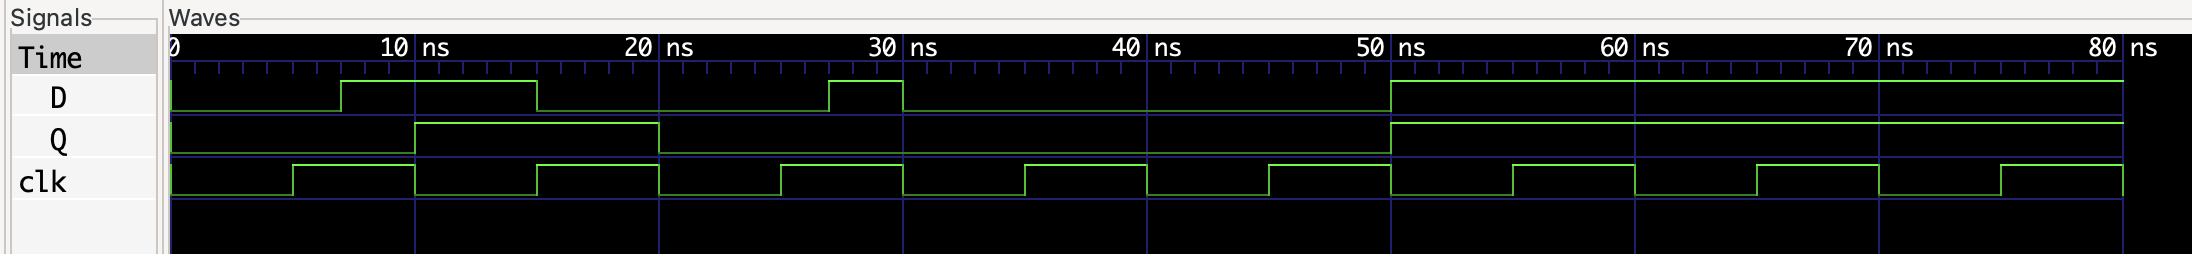
\includegraphics[width=0.8\textwidth]{./verilog_result.png}
	\caption{Verilog simulation waveform of the dfxtn cell}
	\label{fig:dfxtn_verilog_waveform}
\end{figure}

\section{Work Distribution}

\begin{table}[H]
	\centering
	\begin{tabular}{|c|p{10cm}|}
		\hline
		\textbf{Team Members} & \textbf{Contributions}                                                                           \\ \hline
		Bhuvansh              &
		Designed the layout, created the complete .lib file for DFXTN, and prepared the report.                                  \\ \hline
		Saarthak              &
		Calculated characteristics for the combinational circuits, created  Verilog file for the DFXTN, and prepared the report. \\ \hline
		Hardik                &
		Designed the layout for the combinational circuit and calculated the power characteristics for the inverter.             \\ \hline
		Shambhavi             &
		Designed the layout, created the Verilog file, and calculated the timing characteristics for the combinational circuit.  \\ \hline
	\end{tabular}
	\caption{Distribution of work among team members during the project}
	\label{tab:work_distribution}
\end{table}

\end{document}
